% Options for packages loaded elsewhere
\PassOptionsToPackage{unicode}{hyperref}
\PassOptionsToPackage{hyphens}{url}
%
\documentclass[
]{book}
\usepackage{amsmath,amssymb}
\usepackage{iftex}
\ifPDFTeX
  \usepackage[T1]{fontenc}
  \usepackage[utf8]{inputenc}
  \usepackage{textcomp} % provide euro and other symbols
\else % if luatex or xetex
  \usepackage{unicode-math} % this also loads fontspec
  \defaultfontfeatures{Scale=MatchLowercase}
  \defaultfontfeatures[\rmfamily]{Ligatures=TeX,Scale=1}
\fi
\usepackage{lmodern}
\ifPDFTeX\else
  % xetex/luatex font selection
\fi
% Use upquote if available, for straight quotes in verbatim environments
\IfFileExists{upquote.sty}{\usepackage{upquote}}{}
\IfFileExists{microtype.sty}{% use microtype if available
  \usepackage[]{microtype}
  \UseMicrotypeSet[protrusion]{basicmath} % disable protrusion for tt fonts
}{}
\makeatletter
\@ifundefined{KOMAClassName}{% if non-KOMA class
  \IfFileExists{parskip.sty}{%
    \usepackage{parskip}
  }{% else
    \setlength{\parindent}{0pt}
    \setlength{\parskip}{6pt plus 2pt minus 1pt}}
}{% if KOMA class
  \KOMAoptions{parskip=half}}
\makeatother
\usepackage{xcolor}
\usepackage{color}
\usepackage{fancyvrb}
\newcommand{\VerbBar}{|}
\newcommand{\VERB}{\Verb[commandchars=\\\{\}]}
\DefineVerbatimEnvironment{Highlighting}{Verbatim}{commandchars=\\\{\}}
% Add ',fontsize=\small' for more characters per line
\usepackage{framed}
\definecolor{shadecolor}{RGB}{248,248,248}
\newenvironment{Shaded}{\begin{snugshade}}{\end{snugshade}}
\newcommand{\AlertTok}[1]{\textcolor[rgb]{0.94,0.16,0.16}{#1}}
\newcommand{\AnnotationTok}[1]{\textcolor[rgb]{0.56,0.35,0.01}{\textbf{\textit{#1}}}}
\newcommand{\AttributeTok}[1]{\textcolor[rgb]{0.13,0.29,0.53}{#1}}
\newcommand{\BaseNTok}[1]{\textcolor[rgb]{0.00,0.00,0.81}{#1}}
\newcommand{\BuiltInTok}[1]{#1}
\newcommand{\CharTok}[1]{\textcolor[rgb]{0.31,0.60,0.02}{#1}}
\newcommand{\CommentTok}[1]{\textcolor[rgb]{0.56,0.35,0.01}{\textit{#1}}}
\newcommand{\CommentVarTok}[1]{\textcolor[rgb]{0.56,0.35,0.01}{\textbf{\textit{#1}}}}
\newcommand{\ConstantTok}[1]{\textcolor[rgb]{0.56,0.35,0.01}{#1}}
\newcommand{\ControlFlowTok}[1]{\textcolor[rgb]{0.13,0.29,0.53}{\textbf{#1}}}
\newcommand{\DataTypeTok}[1]{\textcolor[rgb]{0.13,0.29,0.53}{#1}}
\newcommand{\DecValTok}[1]{\textcolor[rgb]{0.00,0.00,0.81}{#1}}
\newcommand{\DocumentationTok}[1]{\textcolor[rgb]{0.56,0.35,0.01}{\textbf{\textit{#1}}}}
\newcommand{\ErrorTok}[1]{\textcolor[rgb]{0.64,0.00,0.00}{\textbf{#1}}}
\newcommand{\ExtensionTok}[1]{#1}
\newcommand{\FloatTok}[1]{\textcolor[rgb]{0.00,0.00,0.81}{#1}}
\newcommand{\FunctionTok}[1]{\textcolor[rgb]{0.13,0.29,0.53}{\textbf{#1}}}
\newcommand{\ImportTok}[1]{#1}
\newcommand{\InformationTok}[1]{\textcolor[rgb]{0.56,0.35,0.01}{\textbf{\textit{#1}}}}
\newcommand{\KeywordTok}[1]{\textcolor[rgb]{0.13,0.29,0.53}{\textbf{#1}}}
\newcommand{\NormalTok}[1]{#1}
\newcommand{\OperatorTok}[1]{\textcolor[rgb]{0.81,0.36,0.00}{\textbf{#1}}}
\newcommand{\OtherTok}[1]{\textcolor[rgb]{0.56,0.35,0.01}{#1}}
\newcommand{\PreprocessorTok}[1]{\textcolor[rgb]{0.56,0.35,0.01}{\textit{#1}}}
\newcommand{\RegionMarkerTok}[1]{#1}
\newcommand{\SpecialCharTok}[1]{\textcolor[rgb]{0.81,0.36,0.00}{\textbf{#1}}}
\newcommand{\SpecialStringTok}[1]{\textcolor[rgb]{0.31,0.60,0.02}{#1}}
\newcommand{\StringTok}[1]{\textcolor[rgb]{0.31,0.60,0.02}{#1}}
\newcommand{\VariableTok}[1]{\textcolor[rgb]{0.00,0.00,0.00}{#1}}
\newcommand{\VerbatimStringTok}[1]{\textcolor[rgb]{0.31,0.60,0.02}{#1}}
\newcommand{\WarningTok}[1]{\textcolor[rgb]{0.56,0.35,0.01}{\textbf{\textit{#1}}}}
\usepackage{longtable,booktabs,array}
\usepackage{calc} % for calculating minipage widths
% Correct order of tables after \paragraph or \subparagraph
\usepackage{etoolbox}
\makeatletter
\patchcmd\longtable{\par}{\if@noskipsec\mbox{}\fi\par}{}{}
\makeatother
% Allow footnotes in longtable head/foot
\IfFileExists{footnotehyper.sty}{\usepackage{footnotehyper}}{\usepackage{footnote}}
\makesavenoteenv{longtable}
\usepackage{graphicx}
\makeatletter
\def\maxwidth{\ifdim\Gin@nat@width>\linewidth\linewidth\else\Gin@nat@width\fi}
\def\maxheight{\ifdim\Gin@nat@height>\textheight\textheight\else\Gin@nat@height\fi}
\makeatother
% Scale images if necessary, so that they will not overflow the page
% margins by default, and it is still possible to overwrite the defaults
% using explicit options in \includegraphics[width, height, ...]{}
\setkeys{Gin}{width=\maxwidth,height=\maxheight,keepaspectratio}
% Set default figure placement to htbp
\makeatletter
\def\fps@figure{htbp}
\makeatother
\setlength{\emergencystretch}{3em} % prevent overfull lines
\providecommand{\tightlist}{%
  \setlength{\itemsep}{0pt}\setlength{\parskip}{0pt}}
\setcounter{secnumdepth}{5}
\usepackage{booktabs}
\usepackage{booktabs}
\usepackage{caption}
\usepackage{longtable}
\usepackage{colortbl}
\usepackage{array}
\usepackage{anyfontsize}
\usepackage{multirow}
\ifLuaTeX
  \usepackage{selnolig}  % disable illegal ligatures
\fi
\usepackage[]{natbib}
\bibliographystyle{apalike}
\usepackage{bookmark}
\IfFileExists{xurl.sty}{\usepackage{xurl}}{} % add URL line breaks if available
\urlstyle{same}
\hypersetup{
  pdftitle={Latent Class Analysis with MplusAutomation},
  pdfauthor={Dina Arch},
  hidelinks,
  pdfcreator={LaTeX via pandoc}}

\title{Latent Class Analysis with \texttt{MplusAutomation}}
\author{Dina Arch}
\date{2025-02-13}

\begin{document}
\maketitle

{
\setcounter{tocdepth}{1}
\tableofcontents
}
\chapter*{\texorpdfstring{Mixture Modeling with \texttt{MplusAutomation}}{Mixture Modeling with MplusAutomation}}\label{mixture-modeling-with-mplusautomation}
\addcontentsline{toc}{chapter}{Mixture Modeling with \texttt{MplusAutomation}}

Welcome! This will be a collection of resources that will teach you how to apply mixture modeling using Mplus\citep{muthen2017} and \texttt{MplusAutomation}\citep{hallquist2018}! These resources will serve as a comprehensive guide to understanding and applying LCA using Mplus and its automation capabilities with \texttt{MplusAutomation}. Here, you will learn from start to finish how to apply mixture modeling using Mplus with the \texttt{MplusAutomation} package.

\section*{Stay in touch!}\label{stay-in-touch}
\addcontentsline{toc}{section}{Stay in touch!}

\begin{itemize}
\item
  Please \href{https://immerse.education.ucsb.edu/}{visit our website} to learn more about the IMMERSE fellowship.
\item
  Visit our \href{https://github.com/immerse-ucsb}{GitHub} account to access all the IMMERSE training materials.
\item
  Follow us on \href{https://bsky.app/profile/immerse-ucsb.bsky.social}{BlueSky} and \href{https://twitter.com/IMMERSE_UCSB}{X} to stay-up-to date on our fellowship!
\end{itemize}

\section*{Acknowledgements}\label{acknowledgements}
\addcontentsline{toc}{section}{Acknowledgements}

The Institute of Mixture Modeling for Equity-Oriented Researchers, Scholars, and Educators (IMMERSE) is an IES funded training grant (R305B220021) to support education scholars in integrating mixture modeling into their research.

How to reference this workshop: Institute of Mixture Modeling for Equity-Oriented Researchers, Scholars, and Educators (2025).
IMMERSE Online Resources (IES No.~305B220021).
Institute of Education Sciences.
\url{https://bookdown.org/education_immerse/lca-bookdown/}

\chapter{Introduction to R and RStudio}\label{introduction-to-r-and-rstudio}

\begin{center}\rule{0.5\linewidth}{0.5pt}\end{center}

This walkthrough is presented by the IMMERSE team and will go through some common tasks carried out in R.
There are many free resources available to get started with R and RStudio.
One of our favorites is \href{https://r4ds.had.co.nz/}{\emph{R for Data Science}}.

\begin{center}\rule{0.5\linewidth}{0.5pt}\end{center}

\begin{itemize}
\item
  \emph{R}\citep{rcore2017} is a free, open-source programming language and environment widely used for statistical computing, data analysis, and data visualization.
\item
  \emph{RStudio}\citep{rstudio2020} is an integrated development environment (IDE) for R, providing an intuitive interface that makes coding, visualization, and project management more accessible.
\item
  \emph{Mplus}\citep{muthen2017} is a statistical modeling program used for analyzing complex data, such as latent variable models, structural equation modeling, and growth modeling.
  This book uses an R package called \texttt{MplusAutomation} to automate the process of running models, extracting results, and generating data visualizations.
\end{itemize}

\begin{center}\rule{0.5\linewidth}{0.5pt}\end{center}

\section{Installation}\label{installation}

\begin{center}\rule{0.5\linewidth}{0.5pt}\end{center}

\subsection{Step 0: Install R, RStudio, and Mplus}\label{step-0-install-r-rstudio-and-mplus}

\href{https://posit.co/download/rstudio-desktop/}{Here} you will find a guide to installing both R and R Studio.
You can also install Mplus \href{https://www.statmodel.com/orderonline/}{here}.

\emph{Note}: The installation of Mplus requires a paid license with the mixture add-on.
IMMERSE fellows will be given their own copy of Mplus for use during the one year training.

\begin{center}\rule{0.5\linewidth}{0.5pt}\end{center}

\section{Set-up}\label{set-up}

\begin{center}\rule{0.5\linewidth}{0.5pt}\end{center}

\subsection{Step 1: Create a new R-project in RStudio}\label{step-1-create-a-new-r-project-in-rstudio}

R-projects help us organize our folders , filepaths, and scripts.
To create a new R project:

\begin{itemize}
\tightlist
\item
  File --\textgreater{} New Project\ldots{}
\end{itemize}

Click ``New Directory'' --\textgreater{} New Project --\textgreater{} Name your project

\subsection{Step 2: Create an R-markdown document}\label{step-2-create-an-r-markdown-document}

An R-markdown file provides an authoring framework for data science that allows us to organize our reports using texts and code chunks.
This document you are reading was made using R-markdown!

To create an R-markdown:

\begin{itemize}
\tightlist
\item
  File --\textgreater{} New File --\textgreater{} R Markdown\ldots{}
\end{itemize}

In the window that pops up, give the R-markdown a title such as ``\textbf{Introduction to R and RStudio}'' Click ``OK.'' You should see a new markdown with some example text and code chunks.
We want a clean document to start off with so delete everything from line 10 down.
Go ahead and save this document in your R Project folder.

\subsection{Step 3: Load packages}\label{step-3-load-packages}

Your first code chunk in any given markdown should be the packages you will be using.
To insert a code chunk, etiher use the keyboard shortcut ctrl + alt + i or Code --\textgreater{} Insert Chunk or click the green box with the letter C on it.
There are a few packages we want our markdown to read in:

\begin{Shaded}
\begin{Highlighting}[]
\FunctionTok{library}\NormalTok{(psych) }\CommentTok{\# describe()}
\FunctionTok{library}\NormalTok{(here) }\CommentTok{\#helps with filepaths}
\FunctionTok{library}\NormalTok{(gt) }\CommentTok{\# create tables}
\FunctionTok{library}\NormalTok{(tidyverse) }\CommentTok{\#collection of R packages designed for data science}
\end{Highlighting}
\end{Shaded}

As a reminder, if a function does not work and you receive an error like this: \texttt{could\ not\ find\ function\ "random\_function"}; or if you try to load a package and you receive an error like this: \texttt{there\ is\ no\ package\ called\ \textasciigrave{}random\_package\textasciigrave{}} , then you will need to install the package using \texttt{install.packages("random\_package")} in the console (the bottom-left window in R studio).
Once you have installed the package you will \emph{never} need to install it again, however you must \emph{always} load in the packages at the beginning of your R markdown using \texttt{library(random\_package)}, as shown in this document.

The style of code and package we will be using is called \href{https://www.tidyverse.org/}{\texttt{tidyverse}}\citep{wickham2019} .
Most functions are within the \texttt{tidyverse} package and if not, I've indicated the packages used in the code chunk above.

\begin{center}\rule{0.5\linewidth}{0.5pt}\end{center}

\section{Explore the data}\label{explore-the-data}

\begin{center}\rule{0.5\linewidth}{0.5pt}\end{center}

\subsection{Step 4: Read in data}\label{step-4-read-in-data}

To demonstrate mixture modeling in the training program and online resource components of the IES grant we utilize the \emph{Civil Rights Data Collection (CRDC)} (CRDC) data repository.
The CRDC is a federally mandated school-level data collection effort that occurs every other year.
This public data is currently available for selected latent class indicators across 4 years (2011, 2013, 2015, 2017) and all US states.
In this example, we use the Arizona state sample.
We utilize six focal indicators which constitute the latent class model in our example; three variables which report on harassment/bullying in schools based on disability, race, or sex, and three variables on full-time equivalent school staff hires (counselor, psychologist, law enforcement).
This data source also includes covariates on a variety of subjects and distal outcomes reported in 2018 such as math/reading assessments and graduation rates.

\begin{table}[!t]
\caption*{
{\large LCA indicators\textsuperscript{\textit{1}}}
} 
\fontsize{12.0pt}{14.4pt}\selectfont
\begin{tabular*}{0.75\linewidth}{@{\extracolsep{\fill}}lll}
\toprule
Name & Label & Values \\ 
\midrule\addlinespace[2.5pt]
leaid & District Identification Code &  \\ 
ncessch & School Identification Code &  \\ 
report\_dis & Number of students harassed or bullied on the basis of disability & 0 = No reported incidents, 1 = At least one reported incident \\ 
report\_race & Number of students harassed or bullied on the basis of race, color, or national origin & 0 = No reported incidents, 1 = At least one reported incident \\ 
report\_sex & Number of students harassed or bullied on the basis of sex & 0 = No reported incidents, 1 = At least one reported incident \\ 
counselors\_fte & Number of full time equivalent counselors hired as school staff & 0 = No staff present, 1 = At least one staff present \\ 
report\_sex & Number of full time equivalent psychologists hired as school staff & 0 = No staff present, 1 = At least one staff present \\ 
counselors\_fte & Number of full time equivalent law enforcement officers hired as school staff & 0 = No staff present, 1 = At least one staff present \\ 
\bottomrule
\end{tabular*}
\begin{minipage}{\linewidth}
\textsuperscript{\textit{1}}Civil Rights Data Collection (CRDC)\\
\end{minipage}
\end{table}

\textbf{To read in data in R}:

\begin{Shaded}
\begin{Highlighting}[]
\NormalTok{data }\OtherTok{\textless{}{-}} \FunctionTok{read\_csv}\NormalTok{(}\FunctionTok{here}\NormalTok{(}\StringTok{"data"}\NormalTok{, }\StringTok{"crdc\_lca\_data.csv"}\NormalTok{)) }
\end{Highlighting}
\end{Shaded}

\textbf{Ways to view data in R}:

\begin{enumerate}
\def\labelenumi{\arabic{enumi}.}
\tightlist
\item
  click on the data in your Global Environment (upper right pane) or use\ldots{}
\end{enumerate}

\begin{Shaded}
\begin{Highlighting}[]
\FunctionTok{View}\NormalTok{(data)}
\end{Highlighting}
\end{Shaded}

\begin{enumerate}
\def\labelenumi{\arabic{enumi}.}
\setcounter{enumi}{1}
\tightlist
\item
  \texttt{summary()} gives basic summary statistics \& shows number of NA values (great for checking that data has been read in correctly)
\end{enumerate}

\begin{Shaded}
\begin{Highlighting}[]
\FunctionTok{summary}\NormalTok{(data)}
\CommentTok{\#\textgreater{}     leaid             ncessch            report\_dis    }
\CommentTok{\#\textgreater{}  Length:2027        Length:2027        Min.   :0.0000  }
\CommentTok{\#\textgreater{}  Class :character   Class :character   1st Qu.:0.0000  }
\CommentTok{\#\textgreater{}  Mode  :character   Mode  :character   Median :0.0000  }
\CommentTok{\#\textgreater{}                                        Mean   :0.0425  }
\CommentTok{\#\textgreater{}                                        3rd Qu.:0.0000  }
\CommentTok{\#\textgreater{}                                        Max.   :1.0000  }
\CommentTok{\#\textgreater{}                                        NA\textquotesingle{}s   :27      }
\CommentTok{\#\textgreater{}   report\_race      report\_sex   counselors\_fte  }
\CommentTok{\#\textgreater{}  Min.   :0.000   Min.   :0.00   Min.   :0.0000  }
\CommentTok{\#\textgreater{}  1st Qu.:0.000   1st Qu.:0.00   1st Qu.:0.0000  }
\CommentTok{\#\textgreater{}  Median :0.000   Median :0.00   Median :0.0000  }
\CommentTok{\#\textgreater{}  Mean   :0.103   Mean   :0.17   Mean   :0.4595  }
\CommentTok{\#\textgreater{}  3rd Qu.:0.000   3rd Qu.:0.00   3rd Qu.:1.0000  }
\CommentTok{\#\textgreater{}  Max.   :1.000   Max.   :1.00   Max.   :1.0000  }
\CommentTok{\#\textgreater{}  NA\textquotesingle{}s   :27      NA\textquotesingle{}s   :27     NA\textquotesingle{}s   :27      }
\CommentTok{\#\textgreater{}    psych\_fte         law\_fte      }
\CommentTok{\#\textgreater{}  Min.   :0.0000   Min.   :0.0000  }
\CommentTok{\#\textgreater{}  1st Qu.:0.0000   1st Qu.:0.0000  }
\CommentTok{\#\textgreater{}  Median :0.0000   Median :0.0000  }
\CommentTok{\#\textgreater{}  Mean   :0.4742   Mean   :0.1255  }
\CommentTok{\#\textgreater{}  3rd Qu.:1.0000   3rd Qu.:0.0000  }
\CommentTok{\#\textgreater{}  Max.   :1.0000   Max.   :1.0000  }
\CommentTok{\#\textgreater{}  NA\textquotesingle{}s   :30       NA\textquotesingle{}s   :27}
\end{Highlighting}
\end{Shaded}

\begin{enumerate}
\def\labelenumi{\arabic{enumi}.}
\setcounter{enumi}{2}
\tightlist
\item
  \texttt{names()} provides a list of column names. Very useful if you don't have them memorized!
\end{enumerate}

\begin{Shaded}
\begin{Highlighting}[]
\FunctionTok{names}\NormalTok{(data)}
\CommentTok{\#\textgreater{} [1] "leaid"          "ncessch"        "report\_dis"    }
\CommentTok{\#\textgreater{} [4] "report\_race"    "report\_sex"     "counselors\_fte"}
\CommentTok{\#\textgreater{} [7] "psych\_fte"      "law\_fte"}
\end{Highlighting}
\end{Shaded}

\begin{enumerate}
\def\labelenumi{\arabic{enumi}.}
\setcounter{enumi}{3}
\tightlist
\item
  head() prints the top 6 rows of the dataframe
\end{enumerate}

\begin{Shaded}
\begin{Highlighting}[]
\FunctionTok{head}\NormalTok{(data)}
\CommentTok{\#\textgreater{} \# A tibble: 6 x 8}
\CommentTok{\#\textgreater{}   leaid   ncessch      report\_dis report\_race report\_sex}
\CommentTok{\#\textgreater{}   \textless{}chr\textgreater{}   \textless{}chr\textgreater{}             \textless{}dbl\textgreater{}       \textless{}dbl\textgreater{}      \textless{}dbl\textgreater{}}
\CommentTok{\#\textgreater{} 1 0400001 040000100120          0           0          0}
\CommentTok{\#\textgreater{} 2 0400001 040000100616          0           0          1}
\CommentTok{\#\textgreater{} 3 0400001 040000101204          0           0          1}
\CommentTok{\#\textgreater{} 4 0400001 040000101871          0           1          1}
\CommentTok{\#\textgreater{} 5 0400001 040000101872          0           0          0}
\CommentTok{\#\textgreater{} 6 0400001 040000102344          0           0          0}
\CommentTok{\#\textgreater{} \# i 3 more variables: counselors\_fte \textless{}dbl\textgreater{},}
\CommentTok{\#\textgreater{} \#   psych\_fte \textless{}dbl\textgreater{}, law\_fte \textless{}dbl\textgreater{}}
\end{Highlighting}
\end{Shaded}

\subsection{Step 5: Descriptive Statistics}\label{step-5-descriptive-statistics}

Let's look at descriptive statistics for each variable.
Because looking at the ID variables' (\texttt{leaid}) and (\texttt{necessch}) descriptives is unnecessary, we use \texttt{select()} to remove the variable by using the minus (\texttt{-}) sign:

\begin{Shaded}
\begin{Highlighting}[]
\NormalTok{data }\SpecialCharTok{\%\textgreater{}\%} 
  \FunctionTok{select}\NormalTok{(}\SpecialCharTok{{-}}\NormalTok{leaid, }\SpecialCharTok{{-}}\NormalTok{ncessch) }\SpecialCharTok{\%\textgreater{}\%} 
  \FunctionTok{summary}\NormalTok{()}
\CommentTok{\#\textgreater{}    report\_dis      report\_race      report\_sex  }
\CommentTok{\#\textgreater{}  Min.   :0.0000   Min.   :0.000   Min.   :0.00  }
\CommentTok{\#\textgreater{}  1st Qu.:0.0000   1st Qu.:0.000   1st Qu.:0.00  }
\CommentTok{\#\textgreater{}  Median :0.0000   Median :0.000   Median :0.00  }
\CommentTok{\#\textgreater{}  Mean   :0.0425   Mean   :0.103   Mean   :0.17  }
\CommentTok{\#\textgreater{}  3rd Qu.:0.0000   3rd Qu.:0.000   3rd Qu.:0.00  }
\CommentTok{\#\textgreater{}  Max.   :1.0000   Max.   :1.000   Max.   :1.00  }
\CommentTok{\#\textgreater{}  NA\textquotesingle{}s   :27       NA\textquotesingle{}s   :27      NA\textquotesingle{}s   :27    }
\CommentTok{\#\textgreater{}  counselors\_fte     psych\_fte         law\_fte      }
\CommentTok{\#\textgreater{}  Min.   :0.0000   Min.   :0.0000   Min.   :0.0000  }
\CommentTok{\#\textgreater{}  1st Qu.:0.0000   1st Qu.:0.0000   1st Qu.:0.0000  }
\CommentTok{\#\textgreater{}  Median :0.0000   Median :0.0000   Median :0.0000  }
\CommentTok{\#\textgreater{}  Mean   :0.4595   Mean   :0.4742   Mean   :0.1255  }
\CommentTok{\#\textgreater{}  3rd Qu.:1.0000   3rd Qu.:1.0000   3rd Qu.:0.0000  }
\CommentTok{\#\textgreater{}  Max.   :1.0000   Max.   :1.0000   Max.   :1.0000  }
\CommentTok{\#\textgreater{}  NA\textquotesingle{}s   :27       NA\textquotesingle{}s   :30       NA\textquotesingle{}s   :27}
\end{Highlighting}
\end{Shaded}

Alternatively, we can use the \texttt{psych::describe()} function to give more information:

\begin{Shaded}
\begin{Highlighting}[]
\NormalTok{data }\SpecialCharTok{\%\textgreater{}\%} 
  \FunctionTok{select}\NormalTok{(}\SpecialCharTok{{-}}\NormalTok{leaid, }\SpecialCharTok{{-}}\NormalTok{ncessch) }\SpecialCharTok{\%\textgreater{}\%} 
  \FunctionTok{describe}\NormalTok{()}
\CommentTok{\#\textgreater{}                vars    n mean   sd median trimmed mad min}
\CommentTok{\#\textgreater{} report\_dis        1 2000 0.04 0.20      0    0.00   0   0}
\CommentTok{\#\textgreater{} report\_race       2 2000 0.10 0.30      0    0.00   0   0}
\CommentTok{\#\textgreater{} report\_sex        3 2000 0.17 0.38      0    0.09   0   0}
\CommentTok{\#\textgreater{} counselors\_fte    4 2000 0.46 0.50      0    0.45   0   0}
\CommentTok{\#\textgreater{} psych\_fte         5 1997 0.47 0.50      0    0.47   0   0}
\CommentTok{\#\textgreater{} law\_fte           6 2000 0.13 0.33      0    0.03   0   0}
\CommentTok{\#\textgreater{}                max range skew kurtosis   se}
\CommentTok{\#\textgreater{} report\_dis       1     1 4.53    18.55 0.00}
\CommentTok{\#\textgreater{} report\_race      1     1 2.61     4.82 0.01}
\CommentTok{\#\textgreater{} report\_sex       1     1 1.76     1.08 0.01}
\CommentTok{\#\textgreater{} counselors\_fte   1     1 0.16    {-}1.97 0.01}
\CommentTok{\#\textgreater{} psych\_fte        1     1 0.10    {-}1.99 0.01}
\CommentTok{\#\textgreater{} law\_fte          1     1 2.26     3.11 0.01}
\end{Highlighting}
\end{Shaded}

What if we want to look at a subset of the data?
For example, what if we want to subset the data to observe a specific school district?
(\texttt{leaid}) We can use \texttt{tidyverse::filter()} to subset the data using certain criteria.

\begin{Shaded}
\begin{Highlighting}[]
\NormalTok{data }\SpecialCharTok{\%\textgreater{}\%} 
  \FunctionTok{filter}\NormalTok{(leaid }\SpecialCharTok{==} \StringTok{"0408800"}\NormalTok{) }\SpecialCharTok{\%\textgreater{}\%} 
  \FunctionTok{describe}\NormalTok{() }
\CommentTok{\#\textgreater{}                vars  n  mean    sd median trimmed   mad min}
\CommentTok{\#\textgreater{} leaid*            1 86  1.00  0.00    1.0    1.00  0.00   1}
\CommentTok{\#\textgreater{} ncessch*          2 86 43.50 24.97   43.5   43.50 31.88   1}
\CommentTok{\#\textgreater{} report\_dis        3 86  0.05  0.21    0.0    0.00  0.00   0}
\CommentTok{\#\textgreater{} report\_race       4 86  0.15  0.36    0.0    0.07  0.00   0}
\CommentTok{\#\textgreater{} report\_sex        5 86  0.19  0.39    0.0    0.11  0.00   0}
\CommentTok{\#\textgreater{} counselors\_fte    6 86  0.95  0.21    1.0    1.00  0.00   0}
\CommentTok{\#\textgreater{} psych\_fte         7 86  0.19  0.39    0.0    0.11  0.00   0}
\CommentTok{\#\textgreater{} law\_fte           8 86  0.14  0.35    0.0    0.06  0.00   0}
\CommentTok{\#\textgreater{}                max range  skew kurtosis   se}
\CommentTok{\#\textgreater{} leaid*           1     0   NaN      NaN 0.00}
\CommentTok{\#\textgreater{} ncessch*        86    85  0.00    {-}1.24 2.69}
\CommentTok{\#\textgreater{} report\_dis       1     1  4.23    16.10 0.02}
\CommentTok{\#\textgreater{} report\_race      1     1  1.91     1.68 0.04}
\CommentTok{\#\textgreater{} report\_sex       1     1  1.59     0.52 0.04}
\CommentTok{\#\textgreater{} counselors\_fte   1     1 {-}4.23    16.10 0.02}
\CommentTok{\#\textgreater{} psych\_fte        1     1  1.59     0.52 0.04}
\CommentTok{\#\textgreater{} law\_fte          1     1  2.04     2.21 0.04}


\CommentTok{\#You can use any operator to filter: \textgreater{}, \textless{}, ==, \textgreater{}=, etc.}
\end{Highlighting}
\end{Shaded}

Since we have binary data (0,1), it would be helpful to look at the proportions:

\begin{Shaded}
\begin{Highlighting}[]
\NormalTok{data }\SpecialCharTok{\%\textgreater{}\%} 
  \FunctionTok{drop\_na}\NormalTok{() }\SpecialCharTok{\%\textgreater{}\%} 
  \FunctionTok{pivot\_longer}\NormalTok{(report\_dis}\SpecialCharTok{:}\NormalTok{law\_fte, }\AttributeTok{names\_to =} \StringTok{"variable"}\NormalTok{) }\SpecialCharTok{\%\textgreater{}\%} 
  \FunctionTok{group\_by}\NormalTok{(variable) }\SpecialCharTok{\%\textgreater{}\%} 
  \FunctionTok{summarise}\NormalTok{(}\AttributeTok{prop =} \FunctionTok{sum}\NormalTok{(value)}\SpecialCharTok{/}\FunctionTok{n}\NormalTok{(),}
            \AttributeTok{n =} \FunctionTok{n}\NormalTok{()) }\SpecialCharTok{\%\textgreater{}\%}
  \FunctionTok{arrange}\NormalTok{(}\FunctionTok{desc}\NormalTok{(prop))}
\CommentTok{\#\textgreater{} \# A tibble: 6 x 3}
\CommentTok{\#\textgreater{}   variable         prop     n}
\CommentTok{\#\textgreater{}   \textless{}chr\textgreater{}           \textless{}dbl\textgreater{} \textless{}int\textgreater{}}
\CommentTok{\#\textgreater{} 1 psych\_fte      0.481   1970}
\CommentTok{\#\textgreater{} 2 counselors\_fte 0.459   1970}
\CommentTok{\#\textgreater{} 3 report\_sex     0.173   1970}
\CommentTok{\#\textgreater{} 4 law\_fte        0.127   1970}
\CommentTok{\#\textgreater{} 5 report\_race    0.105   1970}
\CommentTok{\#\textgreater{} 6 report\_dis     0.0431  1970}
\end{Highlighting}
\end{Shaded}

\chapter{\texorpdfstring{Introduction to \texttt{MplusAutomation}}{Introduction to MplusAutomation}}\label{introduction-to-mplusautomation}

\begin{center}\rule{0.5\linewidth}{0.5pt}\end{center}

\texttt{MplusAutomation}\citep{hallquist2018} is designed to streamline the use of Mplus, a powerful statistical software for modeling complex data developed by Muthen and Muten (\url{https://www.statmodel.com}). With \texttt{MplusAutomation}, researchers can automate the process of estimating latent variable models, running batches of models, extracting results, and generating data visualizations - all within the R environment.

\begin{center}\rule{0.5\linewidth}{0.5pt}\end{center}

\textbf{WHAT?}

\begin{itemize}
\tightlist
\item
  \texttt{MplusAutomation} is an \texttt{R} package
\item
  It ``wraps around'' the \texttt{Mplus} program
\item
  Requires both \texttt{R} \& \texttt{Mplus} software
\item
  Requires learning some basics of 2 programming languages
\item
  Car metaphor: R/Rstudio is the \emph{steering wheel or dashboard} \& Mplus is the \emph{engine}
\end{itemize}

\begin{center}\rule{0.5\linewidth}{0.5pt}\end{center}

\textbf{WHY?}

\begin{itemize}
\tightlist
\item
  \texttt{MplusAutomation} can provide clearly organized work procedures in which every research decision can be documented in a single place
\item
  Increase reproducibility, organization, efficiency, and transparency
\end{itemize}

\begin{center}\rule{0.5\linewidth}{0.5pt}\end{center}

\textbf{HOW?}

\begin{itemize}
\tightlist
\item
  The interface for MplusAutomation is entirely within R-Studio. You do not need to open Mplus
\item
  The code presented will be very repetitive by design
\end{itemize}

\begin{center}\rule{0.5\linewidth}{0.5pt}\end{center}

Below is a template for \texttt{mplusObject()} \& \texttt{mplusModeler()} functions. Use this template to run statistical models with Mplus.

\begin{Shaded}
\begin{Highlighting}[]
\NormalTok{m\_template  }\OtherTok{\textless{}{-}} \FunctionTok{mplusObject}\NormalTok{(}
  
  \AttributeTok{TITLE =} 
    \StringTok{""}\NormalTok{, }
  
  \AttributeTok{VARIABLE =} 
    \StringTok{""}\NormalTok{,}
  
  \AttributeTok{ANALYSIS =} 
    \StringTok{""}\NormalTok{,}
  
  \AttributeTok{PLOT =} 
    \StringTok{""}\NormalTok{,}
  
  \AttributeTok{OUTPUT =} 
    \StringTok{""}\NormalTok{,}
 
  \AttributeTok{usevariables =} \FunctionTok{colnames}\NormalTok{(), }
  \AttributeTok{rdata =}\NormalTok{  )}

\NormalTok{m\_template\_fit }\OtherTok{\textless{}{-}} \FunctionTok{mplusModeler}\NormalTok{(m\_template, }
                  \AttributeTok{dataout=}\FunctionTok{here}\NormalTok{(}\StringTok{""}\NormalTok{, }\StringTok{".dat"}\NormalTok{),}
                  \AttributeTok{modelout=}\FunctionTok{here}\NormalTok{(}\StringTok{""}\NormalTok{, }\StringTok{".inp"}\NormalTok{),}
                  \AttributeTok{check=}\ConstantTok{TRUE}\NormalTok{, }\AttributeTok{run =} \ConstantTok{TRUE}\NormalTok{, }\AttributeTok{hashfilename =} \ConstantTok{FALSE}\NormalTok{)}
\end{Highlighting}
\end{Shaded}

\chapter{LCA Enumeration}\label{lca-enumeration}

\begin{center}\rule{0.5\linewidth}{0.5pt}\end{center}

Example: Bullying in Schools

\begin{center}\rule{0.5\linewidth}{0.5pt}\end{center}

To demonstrate mixture modeling in the training program and online resource components of the IES grant we utilize the \emph{Civil Rights Data Collection (CRDC)}\citep{usdoe2014} data repository.
The CRDC is a federally mandated school-level data collection effort that occurs every other year.
This public data is currently available for selected latent class indicators across 4 years (2011, 2013, 2015, 2017) and all US states.
In this example, we use the Arizona state sample.
We utilize six focal indicators which constitute the latent class model in our example; three variables which report on harassment/bullying in schools based on disability, race, or sex, and three variables on full-time equivalent school staff hires (counselor, psychologist, law enforcement).
This data source also includes covariates on a variety of subjects and distal outcomes reported in 2018 such as math/reading assessments and graduation rates.

\begin{center}\rule{0.5\linewidth}{0.5pt}\end{center}

Load packages

\begin{Shaded}
\begin{Highlighting}[]
\FunctionTok{library}\NormalTok{(tidyverse)}
\FunctionTok{library}\NormalTok{(haven)}
\FunctionTok{library}\NormalTok{(glue)}
\FunctionTok{library}\NormalTok{(MplusAutomation)}
\FunctionTok{library}\NormalTok{(here)}
\FunctionTok{library}\NormalTok{(janitor)}
\FunctionTok{library}\NormalTok{(gt)}
\FunctionTok{library}\NormalTok{(cowplot)}
\FunctionTok{library}\NormalTok{(DiagrammeR) }
\end{Highlighting}
\end{Shaded}

\section{Variable Description}\label{variable-description}

\begin{table}[!t]
\caption*{
{\large LCA indicators\textsuperscript{\textit{1}}}
} 
\fontsize{12.0pt}{14.4pt}\selectfont
\begin{tabular*}{0.75\linewidth}{@{\extracolsep{\fill}}lll}
\toprule
Name & Label & Values \\ 
\midrule\addlinespace[2.5pt]
leaid & District Identification Code &  \\ 
ncessch & School Identification Code &  \\ 
report\_dis & Number of students harassed or bullied on the basis of disability & 0 = No reported incidents, 1 = At least one reported incident \\ 
report\_race & Number of students harassed or bullied on the basis of race, color, or national origin & 0 = No reported incidents, 1 = At least one reported incident \\ 
report\_sex & Number of students harassed or bullied on the basis of sex & 0 = No reported incidents, 1 = At least one reported incident \\ 
counselors\_fte & Number of full time equivalent counselors hired as school staff & 0 = No staff present, 1 = At least one staff present \\ 
psych\_fte & Number of full time equivalent psychologists hired as school staff & 0 = No staff present, 1 = At least one staff present \\ 
law\_fte & Number of full time equivalent law enforcement officers hired as school staff & 0 = No staff present, 1 = At least one staff present \\ 
\bottomrule
\end{tabular*}
\begin{minipage}{\linewidth}
\textsuperscript{\textit{1}}Civil Rights Data Collection (CRDC)\\
\end{minipage}
\end{table}

\begin{center}\rule{0.5\linewidth}{0.5pt}\end{center}

\textbf{Variables have been transformed to be dichotomous indicators using the following coding strategy}

Harassment and bullying count variables are recoded \texttt{1} if the school reported at least one incident of harassment (\texttt{0} indicates no reported incidents).
On the original scale reported by the CDRC staff variables for full time equivalent employees (FTE) are represented as \texttt{1} and part time employees are represented by values between \texttt{1} and \texttt{0}.
Schools with greater than one staff of the designated type are represented by values greater than 1.
All values greater than zero were recorded as \texttt{1s} (e.g., \texttt{.5}, \texttt{1},\texttt{3}) indicating that the school has a staff present on campus at least part time.
Schools with no staff of the designated type are indicated as \texttt{0} for the dichotomous variable.

\begin{center}\rule{0.5\linewidth}{0.5pt}\end{center}

\begin{center}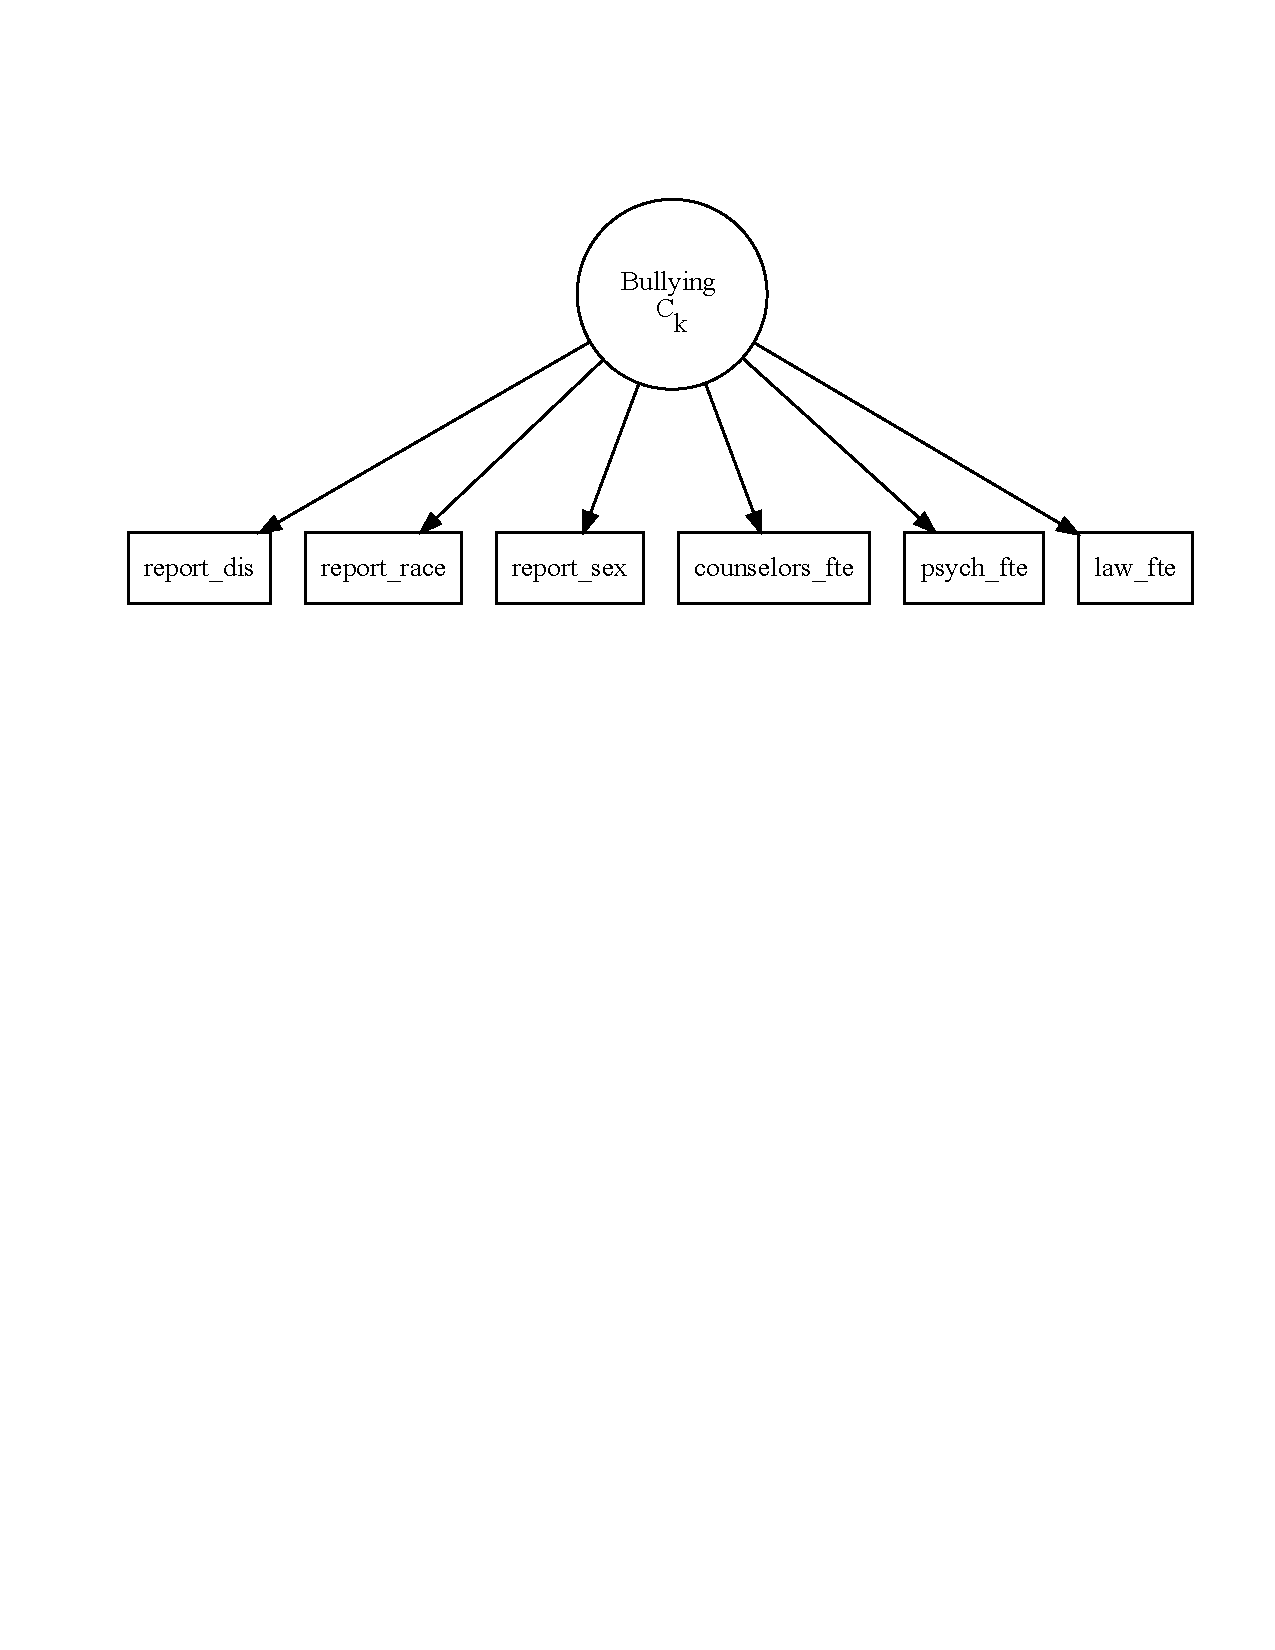
\includegraphics{03-enumeration_files/figure-latex/unnamed-chunk-3-1} \end{center}

\begin{center}\rule{0.5\linewidth}{0.5pt}\end{center}

\section{Prepare Data}\label{prepare-data}

\begin{Shaded}
\begin{Highlighting}[]
\NormalTok{df\_bully }\OtherTok{\textless{}{-}} \FunctionTok{read\_csv}\NormalTok{(}\FunctionTok{here}\NormalTok{(}\StringTok{"data"}\NormalTok{, }\StringTok{"crdc\_lca\_data.csv"}\NormalTok{)) }\SpecialCharTok{\%\textgreater{}\%} 
  \FunctionTok{clean\_names}\NormalTok{() }\SpecialCharTok{\%\textgreater{}\%} 
\NormalTok{  dplyr}\SpecialCharTok{::}\FunctionTok{select}\NormalTok{(report\_dis, report\_race, report\_sex, counselors\_fte, psych\_fte, law\_fte) }
\end{Highlighting}
\end{Shaded}

\begin{center}\rule{0.5\linewidth}{0.5pt}\end{center}

\section{Descriptive Statistics}\label{descriptive-statistics}

\begin{Shaded}
\begin{Highlighting}[]
\CommentTok{\# Set up data to find proportions of binary indicators}
\NormalTok{ds }\OtherTok{\textless{}{-}}\NormalTok{ df\_bully }\SpecialCharTok{\%\textgreater{}\%} 
  \FunctionTok{pivot\_longer}\NormalTok{(}\FunctionTok{c}\NormalTok{(report\_dis, report\_race, report\_sex, counselors\_fte, psych\_fte, law\_fte), }\AttributeTok{names\_to =} \StringTok{"variable"}\NormalTok{) }


\CommentTok{\# Create table of variables and counts, then find proportions and round to 3 decimal places}
\NormalTok{prop\_df }\OtherTok{\textless{}{-}}\NormalTok{ ds }\SpecialCharTok{\%\textgreater{}\%}
  \FunctionTok{count}\NormalTok{(variable, value) }\SpecialCharTok{\%\textgreater{}\%}
  \FunctionTok{group\_by}\NormalTok{(variable) }\SpecialCharTok{\%\textgreater{}\%}
  \FunctionTok{mutate}\NormalTok{(}\AttributeTok{prop =}\NormalTok{ n }\SpecialCharTok{/} \FunctionTok{sum}\NormalTok{(n)) }\SpecialCharTok{\%\textgreater{}\%}
  \FunctionTok{ungroup}\NormalTok{() }\SpecialCharTok{\%\textgreater{}\%}
  \FunctionTok{mutate}\NormalTok{(}\AttributeTok{prop =} \FunctionTok{round}\NormalTok{(prop, }\DecValTok{3}\NormalTok{))}


\CommentTok{\# Make it a gt() table}
\NormalTok{prop\_table }\OtherTok{\textless{}{-}}\NormalTok{ prop\_df }\SpecialCharTok{\%\textgreater{}\%} 
  \FunctionTok{gt}\NormalTok{(}\AttributeTok{groupname\_col =} \StringTok{"variable"}\NormalTok{, }\AttributeTok{rowname\_col =} \StringTok{"value"}\NormalTok{) }\SpecialCharTok{\%\textgreater{}\%}
  \FunctionTok{tab\_stubhead}\NormalTok{(}\AttributeTok{label =} \FunctionTok{md}\NormalTok{(}\StringTok{"*Values*"}\NormalTok{)) }\SpecialCharTok{\%\textgreater{}\%}
  \FunctionTok{tab\_header}\NormalTok{(}
    \FunctionTok{md}\NormalTok{(}
      \StringTok{"Variable Proportions"}
\NormalTok{    )}
\NormalTok{  ) }\SpecialCharTok{\%\textgreater{}\%}
  \FunctionTok{cols\_label}\NormalTok{(}
    \AttributeTok{variable =} \FunctionTok{md}\NormalTok{(}\StringTok{"*Variable*"}\NormalTok{),}
    \AttributeTok{value =} \FunctionTok{md}\NormalTok{(}\StringTok{"*Value*"}\NormalTok{),}
    \AttributeTok{n =} \FunctionTok{md}\NormalTok{(}\StringTok{"*N*"}\NormalTok{),}
    \AttributeTok{prop =} \FunctionTok{md}\NormalTok{(}\StringTok{"*Proportion*"}\NormalTok{)}
\NormalTok{  ) }
  
\NormalTok{prop\_table}
\end{Highlighting}
\end{Shaded}

\begin{table}[!t]
\caption*{
{\large Variable Proportions}
} 
\fontsize{12.0pt}{14.4pt}\selectfont
\begin{tabular*}{\linewidth}{@{\extracolsep{\fill}}l|rr}
\toprule
\emph{Values} & \emph{N} & \emph{Proportion} \\ 
\midrule\addlinespace[2.5pt]
\multicolumn{3}{l}{counselors\_fte} \\[2.5pt] 
\midrule\addlinespace[2.5pt]
0 & 1081 & 0.533 \\ 
1 & 919 & 0.453 \\ 
NA & 27 & 0.013 \\ 
\midrule\addlinespace[2.5pt]
\multicolumn{3}{l}{law\_fte} \\[2.5pt] 
\midrule\addlinespace[2.5pt]
0 & 1749 & 0.863 \\ 
1 & 251 & 0.124 \\ 
NA & 27 & 0.013 \\ 
\midrule\addlinespace[2.5pt]
\multicolumn{3}{l}{psych\_fte} \\[2.5pt] 
\midrule\addlinespace[2.5pt]
0 & 1050 & 0.518 \\ 
1 & 947 & 0.467 \\ 
NA & 30 & 0.015 \\ 
\midrule\addlinespace[2.5pt]
\multicolumn{3}{l}{report\_dis} \\[2.5pt] 
\midrule\addlinespace[2.5pt]
0 & 1915 & 0.945 \\ 
1 & 85 & 0.042 \\ 
NA & 27 & 0.013 \\ 
\midrule\addlinespace[2.5pt]
\multicolumn{3}{l}{report\_race} \\[2.5pt] 
\midrule\addlinespace[2.5pt]
0 & 1794 & 0.885 \\ 
1 & 206 & 0.102 \\ 
NA & 27 & 0.013 \\ 
\midrule\addlinespace[2.5pt]
\multicolumn{3}{l}{report\_sex} \\[2.5pt] 
\midrule\addlinespace[2.5pt]
0 & 1660 & 0.819 \\ 
1 & 340 & 0.168 \\ 
NA & 27 & 0.013 \\ 
\bottomrule
\end{tabular*}
\end{table}

Save as image

\begin{Shaded}
\begin{Highlighting}[]
\FunctionTok{gtsave}\NormalTok{(prop\_table, }\FunctionTok{here}\NormalTok{(}\StringTok{"figures"}\NormalTok{, }\StringTok{"prop\_table.png"}\NormalTok{))}
\end{Highlighting}
\end{Shaded}

\begin{center}\rule{0.5\linewidth}{0.5pt}\end{center}

\section{Enumeration}\label{enumeration}

This code uses the \texttt{mplusObject} function in the \texttt{MplusAutomation} package and saves all model runs in the \texttt{enum} folder.

\begin{Shaded}
\begin{Highlighting}[]

\NormalTok{lca\_6  }\OtherTok{\textless{}{-}} \FunctionTok{lapply}\NormalTok{(}\DecValTok{1}\SpecialCharTok{:}\DecValTok{6}\NormalTok{, }\ControlFlowTok{function}\NormalTok{(k) \{}
\NormalTok{  lca\_enum  }\OtherTok{\textless{}{-}} \FunctionTok{mplusObject}\NormalTok{(}
      
    \AttributeTok{TITLE =} \FunctionTok{glue}\NormalTok{(}\StringTok{"\{k\}{-}Class"}\NormalTok{), }
  
    \AttributeTok{VARIABLE =} \FunctionTok{glue}\NormalTok{(}
    \StringTok{"categorical = report\_dis{-}law\_fte; }
\StringTok{     usevar = report\_dis{-}law\_fte;}
\StringTok{     classes = c(\{k\}); "}\NormalTok{),}
  
  \AttributeTok{ANALYSIS =} 
   \StringTok{"estimator = mlr; }
\StringTok{    type = mixture;}
\StringTok{    starts = 200 100; }
\StringTok{    processors = 10;"}\NormalTok{,}
  
  \AttributeTok{OUTPUT =} \StringTok{"sampstat residual tech11 tech14;"}\NormalTok{,}
  
  \AttributeTok{PLOT =} 
    \StringTok{"type = plot3; }
\StringTok{    series = report\_dis{-}law\_fte(*);"}\NormalTok{,}
  
  \AttributeTok{usevariables =} \FunctionTok{colnames}\NormalTok{(df\_bully),}
  \AttributeTok{rdata =}\NormalTok{ df\_bully)}

\NormalTok{lca\_enum\_fit }\OtherTok{\textless{}{-}} \FunctionTok{mplusModeler}\NormalTok{(lca\_enum, }
                            \AttributeTok{dataout=}\FunctionTok{glue}\NormalTok{(}\FunctionTok{here}\NormalTok{(}\StringTok{"enum"}\NormalTok{, }\StringTok{"bully.dat"}\NormalTok{)),}
                            \AttributeTok{modelout=}\FunctionTok{glue}\NormalTok{(}\FunctionTok{here}\NormalTok{(}\StringTok{"enum"}\NormalTok{, }\StringTok{"c\{k\}\_bully.inp"}\NormalTok{)) ,}
                            \AttributeTok{check=}\ConstantTok{TRUE}\NormalTok{, }\AttributeTok{run =} \ConstantTok{TRUE}\NormalTok{, }\AttributeTok{hashfilename =} \ConstantTok{FALSE}\NormalTok{)}
\NormalTok{\})}
\end{Highlighting}
\end{Shaded}

\textbf{IMPORTANT}: Before moving forward, make sure to open each output document to ensure models were estimated normally.

\begin{center}\rule{0.5\linewidth}{0.5pt}\end{center}

\section{Table of Fit}\label{table-of-fit}

First, extract data:

\begin{Shaded}
\begin{Highlighting}[]
\CommentTok{\# }
\NormalTok{output\_bully }\OtherTok{\textless{}{-}} \FunctionTok{readModels}\NormalTok{(}\FunctionTok{here}\NormalTok{(}\StringTok{"enum"}\NormalTok{), }\AttributeTok{filefilter =} \StringTok{"bully"}\NormalTok{, }\AttributeTok{quiet =} \ConstantTok{TRUE}\NormalTok{)}

\NormalTok{enum\_extract }\OtherTok{\textless{}{-}} \FunctionTok{LatexSummaryTable}\NormalTok{(}
\NormalTok{  output\_bully,}
  \AttributeTok{keepCols =} \FunctionTok{c}\NormalTok{(}
    \StringTok{"Title"}\NormalTok{,}
    \StringTok{"Parameters"}\NormalTok{,}
    \StringTok{"LL"}\NormalTok{,}
    \StringTok{"BIC"}\NormalTok{,}
    \StringTok{"aBIC"}\NormalTok{,}
    \StringTok{"BLRT\_PValue"}\NormalTok{,}
    \StringTok{"T11\_VLMR\_PValue"}\NormalTok{,}
    \StringTok{"Observations"}
\NormalTok{  ),}
  \AttributeTok{sortBy =} \StringTok{"Title"}
\NormalTok{) }


\NormalTok{allFit }\OtherTok{\textless{}{-}}\NormalTok{ enum\_extract }\SpecialCharTok{\%\textgreater{}\%}
  \FunctionTok{mutate}\NormalTok{(}\AttributeTok{CAIC =} \SpecialCharTok{{-}}\DecValTok{2} \SpecialCharTok{*}\NormalTok{ LL }\SpecialCharTok{+}\NormalTok{ Parameters }\SpecialCharTok{*}\NormalTok{ (}\FunctionTok{log}\NormalTok{(Observations) }\SpecialCharTok{+} \DecValTok{1}\NormalTok{)) }\SpecialCharTok{\%\textgreater{}\%}
  \FunctionTok{mutate}\NormalTok{(}\AttributeTok{AWE =} \SpecialCharTok{{-}}\DecValTok{2} \SpecialCharTok{*}\NormalTok{ LL }\SpecialCharTok{+} \DecValTok{2} \SpecialCharTok{*}\NormalTok{ Parameters }\SpecialCharTok{*}\NormalTok{ (}\FunctionTok{log}\NormalTok{(Observations) }\SpecialCharTok{+} \FloatTok{1.5}\NormalTok{)) }\SpecialCharTok{\%\textgreater{}\%}
  \FunctionTok{mutate}\NormalTok{(}\AttributeTok{SIC =} \SpecialCharTok{{-}}\NormalTok{.}\DecValTok{5} \SpecialCharTok{*}\NormalTok{ BIC) }\SpecialCharTok{\%\textgreater{}\%}
  \FunctionTok{mutate}\NormalTok{(}\AttributeTok{expSIC =} \FunctionTok{exp}\NormalTok{(SIC }\SpecialCharTok{{-}} \FunctionTok{max}\NormalTok{(SIC))) }\SpecialCharTok{\%\textgreater{}\%}
  \FunctionTok{mutate}\NormalTok{(}\AttributeTok{BF =} \FunctionTok{exp}\NormalTok{(SIC }\SpecialCharTok{{-}} \FunctionTok{lead}\NormalTok{(SIC))) }\SpecialCharTok{\%\textgreater{}\%}
  \FunctionTok{mutate}\NormalTok{(}\AttributeTok{cmPk =}\NormalTok{ expSIC }\SpecialCharTok{/} \FunctionTok{sum}\NormalTok{(expSIC)) }\SpecialCharTok{\%\textgreater{}\%}
\NormalTok{  dplyr}\SpecialCharTok{::}\FunctionTok{select}\NormalTok{(}\DecValTok{1}\SpecialCharTok{:}\DecValTok{5}\NormalTok{, }\DecValTok{9}\SpecialCharTok{:}\DecValTok{10}\NormalTok{, }\DecValTok{6}\SpecialCharTok{:}\DecValTok{7}\NormalTok{, }\DecValTok{13}\NormalTok{, }\DecValTok{14}\NormalTok{) }\SpecialCharTok{\%\textgreater{}\%}
  \FunctionTok{arrange}\NormalTok{(Parameters)}
\end{Highlighting}
\end{Shaded}

Then, create table:

\begin{Shaded}
\begin{Highlighting}[]
\NormalTok{fit\_table1 }\OtherTok{\textless{}{-}}\NormalTok{ allFit }\SpecialCharTok{\%\textgreater{}\%}
  \FunctionTok{gt}\NormalTok{() }\SpecialCharTok{\%\textgreater{}\%}
  \FunctionTok{tab\_header}\NormalTok{(}\AttributeTok{title =} \FunctionTok{md}\NormalTok{(}\StringTok{"**Model Fit Summary Table**"}\NormalTok{)) }\SpecialCharTok{\%\textgreater{}\%}
  \FunctionTok{cols\_label}\NormalTok{(}
    \AttributeTok{Title =} \StringTok{"Classes"}\NormalTok{,}
    \AttributeTok{Parameters =} \FunctionTok{md}\NormalTok{(}\StringTok{"Par"}\NormalTok{),}
    \AttributeTok{LL =} \FunctionTok{md}\NormalTok{(}\StringTok{"*LL*"}\NormalTok{),}
    \AttributeTok{T11\_VLMR\_PValue =} \StringTok{"VLMR"}\NormalTok{,}
    \AttributeTok{BLRT\_PValue =} \StringTok{"BLRT"}\NormalTok{,}
    \AttributeTok{BF =} \FunctionTok{md}\NormalTok{(}\StringTok{"BF"}\NormalTok{),}
    \AttributeTok{cmPk =} \FunctionTok{md}\NormalTok{(}\StringTok{"*cmPk*"}\NormalTok{)}
\NormalTok{  ) }\SpecialCharTok{\%\textgreater{}\%}
  \FunctionTok{tab\_footnote}\NormalTok{(}
    \AttributeTok{footnote =} \FunctionTok{md}\NormalTok{(}
      \StringTok{"*Note.* Par = Parameters; *LL* = model log likelihood;}
\StringTok{BIC = Bayesian information criterion;}
\StringTok{aBIC = sample size adjusted BIC; CAIC = consistent Akaike information criterion;}
\StringTok{AWE = approximate weight of evidence criterion;}
\StringTok{BLRT = bootstrapped likelihood ratio test p{-}value;}
\StringTok{VLMR = Vuong{-}Lo{-}Mendell{-}Rubin adjusted likelihood ratio test p{-}value;}
\StringTok{*cmPk* = approximate correct model probability."}
\NormalTok{    ),}
\AttributeTok{locations =} \FunctionTok{cells\_title}\NormalTok{()}
\NormalTok{  ) }\SpecialCharTok{\%\textgreater{}\%}
  \FunctionTok{tab\_options}\NormalTok{(}\AttributeTok{column\_labels.font.weight =} \StringTok{"bold"}\NormalTok{) }\SpecialCharTok{\%\textgreater{}\%}
  \FunctionTok{fmt\_number}\NormalTok{(}\FunctionTok{c}\NormalTok{(}\DecValTok{3}\SpecialCharTok{:}\DecValTok{7}\NormalTok{),}
             \AttributeTok{decimals =} \DecValTok{2}\NormalTok{) }\SpecialCharTok{\%\textgreater{}\%}
  \FunctionTok{sub\_missing}\NormalTok{(}\DecValTok{1}\SpecialCharTok{:}\DecValTok{11}\NormalTok{,}
              \AttributeTok{missing\_text =} \StringTok{"{-}{-}"}\NormalTok{) }\SpecialCharTok{\%\textgreater{}\%}
  \FunctionTok{fmt}\NormalTok{(}
    \FunctionTok{c}\NormalTok{(}\DecValTok{8}\SpecialCharTok{:}\DecValTok{9}\NormalTok{, }\DecValTok{11}\NormalTok{),}
    \AttributeTok{fns =} \ControlFlowTok{function}\NormalTok{(x)}
      \FunctionTok{ifelse}\NormalTok{(x }\SpecialCharTok{\textless{}} \FloatTok{0.001}\NormalTok{, }\StringTok{"\textless{}.001"}\NormalTok{,}
\NormalTok{             scales}\SpecialCharTok{::}\FunctionTok{number}\NormalTok{(x, }\AttributeTok{accuracy =}\NormalTok{ .}\DecValTok{01}\NormalTok{))}
\NormalTok{  ) }\SpecialCharTok{\%\textgreater{}\%}
  \FunctionTok{fmt}\NormalTok{(}
    \DecValTok{10}\NormalTok{,}
    \AttributeTok{fns =} \ControlFlowTok{function}\NormalTok{ (x)}
      \FunctionTok{ifelse}\NormalTok{(x }\SpecialCharTok{\textgreater{}} \DecValTok{100}\NormalTok{, }\StringTok{"\textgreater{}100"}\NormalTok{,}
\NormalTok{             scales}\SpecialCharTok{::}\FunctionTok{number}\NormalTok{(x, }\AttributeTok{accuracy =}\NormalTok{ .}\DecValTok{01}\NormalTok{))}
\NormalTok{  ) }\SpecialCharTok{\%\textgreater{}\%}  
  \FunctionTok{tab\_style}\NormalTok{(}
    \AttributeTok{style =} \FunctionTok{list}\NormalTok{(}
      \FunctionTok{cell\_text}\NormalTok{(}\AttributeTok{weight =} \StringTok{"bold"}\NormalTok{)}
\NormalTok{      ),}
    \AttributeTok{locations =} \FunctionTok{list}\NormalTok{(}\FunctionTok{cells\_body}\NormalTok{(}
     \AttributeTok{columns =}\NormalTok{ BIC,}
     \AttributeTok{row =}\NormalTok{ BIC }\SpecialCharTok{==} \FunctionTok{min}\NormalTok{(BIC[}\FunctionTok{c}\NormalTok{(}\DecValTok{1}\SpecialCharTok{:}\DecValTok{6}\NormalTok{)]) }\CommentTok{\# Change this to the number of classes you are evaluating}
\NormalTok{    ),}
    \FunctionTok{cells\_body}\NormalTok{(}
     \AttributeTok{columns =}\NormalTok{ aBIC,}
     \AttributeTok{row =}\NormalTok{ aBIC }\SpecialCharTok{==} \FunctionTok{min}\NormalTok{(aBIC[}\DecValTok{1}\SpecialCharTok{:}\DecValTok{6}\NormalTok{])}
\NormalTok{    ),}
    \FunctionTok{cells\_body}\NormalTok{(}
     \AttributeTok{columns =}\NormalTok{ CAIC,}
     \AttributeTok{row =}\NormalTok{ CAIC }\SpecialCharTok{==} \FunctionTok{min}\NormalTok{(CAIC[}\DecValTok{1}\SpecialCharTok{:}\DecValTok{6}\NormalTok{])}
\NormalTok{    ),}
    \FunctionTok{cells\_body}\NormalTok{(}
     \AttributeTok{columns =}\NormalTok{ AWE,}
     \AttributeTok{row =}\NormalTok{ AWE }\SpecialCharTok{==} \FunctionTok{min}\NormalTok{(AWE[}\DecValTok{1}\SpecialCharTok{:}\DecValTok{6}\NormalTok{])}
\NormalTok{    ),}
    \FunctionTok{cells\_body}\NormalTok{(}
     \AttributeTok{columns =}\NormalTok{ cmPk,}
     \AttributeTok{row =}\NormalTok{  cmPk }\SpecialCharTok{==} \FunctionTok{max}\NormalTok{(cmPk[}\DecValTok{1}\SpecialCharTok{:}\DecValTok{6}\NormalTok{])}
\NormalTok{     ),    }
    \FunctionTok{cells\_body}\NormalTok{(}
     \AttributeTok{columns =}\NormalTok{ BF,}
     \AttributeTok{row =}\NormalTok{  BF }\SpecialCharTok{\textgreater{}} \DecValTok{10}\NormalTok{),}
    \FunctionTok{cells\_body}\NormalTok{( }
     \AttributeTok{columns =}\NormalTok{  T11\_VLMR\_PValue,}
     \AttributeTok{row =}  \FunctionTok{ifelse}\NormalTok{(T11\_VLMR\_PValue }\SpecialCharTok{\textless{}}\NormalTok{ .}\DecValTok{05} \SpecialCharTok{\&} \FunctionTok{lead}\NormalTok{(T11\_VLMR\_PValue) }\SpecialCharTok{\textgreater{}}\NormalTok{ .}\DecValTok{05}\NormalTok{, T11\_VLMR\_PValue }\SpecialCharTok{\textless{}}\NormalTok{ .}\DecValTok{05}\NormalTok{, }\ConstantTok{NA}\NormalTok{)),}
    \FunctionTok{cells\_body}\NormalTok{(}
     \AttributeTok{columns =}\NormalTok{  BLRT\_PValue,}
     \AttributeTok{row =}  \FunctionTok{ifelse}\NormalTok{(BLRT\_PValue }\SpecialCharTok{\textless{}}\NormalTok{ .}\DecValTok{05} \SpecialCharTok{\&} \FunctionTok{lead}\NormalTok{(BLRT\_PValue) }\SpecialCharTok{\textgreater{}}\NormalTok{ .}\DecValTok{05}\NormalTok{, BLRT\_PValue }\SpecialCharTok{\textless{}}\NormalTok{ .}\DecValTok{05}\NormalTok{, }\ConstantTok{NA}\NormalTok{))}
\NormalTok{  )}
\NormalTok{)}

\NormalTok{fit\_table1}
\end{Highlighting}
\end{Shaded}

\begin{table}[!t]
\caption*{
{\large \textbf{Model Fit Summary Table}\textsuperscript{\textit{1}}}
} 
\fontsize{12.0pt}{14.4pt}\selectfont
\begin{tabular*}{\linewidth}{@{\extracolsep{\fill}}lrrrrrrrrrr}
\toprule
Classes & Par & \emph{LL} & BIC & aBIC & CAIC & AWE & BLRT & VLMR & BF & \emph{cmPk} \\ 
\midrule\addlinespace[2.5pt]
1-Class & 6 & -5,443.41 & 10,932.50 & 10,913.44 & 10,938.50 & 10,996.19 & – & – & 0.00 & <.001 \\ 
2-Class & 13 & -5,194.14 & 10,487.26 & 10,445.96 & 10,500.26 & 10,625.24 & <.001 & <.001 & 0.00 & <.001 \\ 
3-Class & 20 & -5,122.48 & {\bfseries 10,397.24} & {\bfseries 10,333.70} & {\bfseries 10,417.24} & {\bfseries 10,609.53} & <.001 & <.001 & {\bfseries >100} & {\bfseries 1.00} \\ 
4-Class & 27 & -5,111.76 & 10,429.10 & 10,343.32 & 10,456.10 & 10,715.69 & {\bfseries <.001} & {\bfseries 0.01} & {\bfseries >100} & <.001 \\ 
5-Class & 34 & -5,105.59 & 10,470.07 & 10,362.04 & 10,504.06 & 10,830.95 & 0.29 & 0.18 & {\bfseries >100} & <.001 \\ 
6-Class & 41 & -5,099.88 & 10,511.95 & 10,381.69 & 10,552.95 & 10,947.14 & 0.38 & 0.18 & – & <.001 \\ 
\bottomrule
\end{tabular*}
\begin{minipage}{\linewidth}
\textsuperscript{\textit{1}}\emph{Note.} Par = Parameters; \emph{LL} = model log likelihood;
BIC = Bayesian information criterion;
aBIC = sample size adjusted BIC; CAIC = consistent Akaike information criterion;
AWE = approximate weight of evidence criterion;
BLRT = bootstrapped likelihood ratio test p-value;
VLMR = Vuong-Lo-Mendell-Rubin adjusted likelihood ratio test p-value;
\emph{cmPk} = approximate correct model probability.\\
\end{minipage}
\end{table}

\begin{center}\rule{0.5\linewidth}{0.5pt}\end{center}

Save table

\begin{Shaded}
\begin{Highlighting}[]
\FunctionTok{gtsave}\NormalTok{(fit\_table1, }\FunctionTok{here}\NormalTok{(}\StringTok{"figures"}\NormalTok{, }\StringTok{"fit\_table.png"}\NormalTok{))}
\end{Highlighting}
\end{Shaded}

\begin{center}\rule{0.5\linewidth}{0.5pt}\end{center}

\section{Information Criteria Plot}\label{information-criteria-plot}

\begin{Shaded}
\begin{Highlighting}[]
\NormalTok{allFit }\SpecialCharTok{\%\textgreater{}\%}
\NormalTok{  dplyr}\SpecialCharTok{::}\FunctionTok{select}\NormalTok{(}\DecValTok{2}\SpecialCharTok{:}\DecValTok{7}\NormalTok{) }\SpecialCharTok{\%\textgreater{}\%}
  \FunctionTok{rowid\_to\_column}\NormalTok{() }\SpecialCharTok{\%\textgreater{}\%}
  \FunctionTok{pivot\_longer}\NormalTok{(}\StringTok{\textasciigrave{}}\AttributeTok{BIC}\StringTok{\textasciigrave{}}\SpecialCharTok{:}\StringTok{\textasciigrave{}}\AttributeTok{AWE}\StringTok{\textasciigrave{}}\NormalTok{,}
               \AttributeTok{names\_to =} \StringTok{"Index"}\NormalTok{,}
               \AttributeTok{values\_to =} \StringTok{"ic\_value"}\NormalTok{) }\SpecialCharTok{\%\textgreater{}\%}
  \FunctionTok{mutate}\NormalTok{(}\AttributeTok{Index =} \FunctionTok{factor}\NormalTok{(Index,}
                        \AttributeTok{levels =} \FunctionTok{c}\NormalTok{ (}\StringTok{"AWE"}\NormalTok{, }\StringTok{"CAIC"}\NormalTok{, }\StringTok{"BIC"}\NormalTok{, }\StringTok{"aBIC"}\NormalTok{))) }\SpecialCharTok{\%\textgreater{}\%}
  \FunctionTok{ggplot}\NormalTok{(}\FunctionTok{aes}\NormalTok{(}
    \AttributeTok{x =}\NormalTok{ rowid,}
    \AttributeTok{y =}\NormalTok{ ic\_value,}
    \AttributeTok{color =}\NormalTok{ Index,}
    \AttributeTok{shape =}\NormalTok{ Index,}
    \AttributeTok{group =}\NormalTok{ Index,}
    \AttributeTok{lty =}\NormalTok{ Index}
\NormalTok{  )) }\SpecialCharTok{+}
  \FunctionTok{geom\_point}\NormalTok{(}\AttributeTok{size =} \FloatTok{2.0}\NormalTok{) }\SpecialCharTok{+} \FunctionTok{geom\_line}\NormalTok{(}\AttributeTok{linewidth =}\NormalTok{ .}\DecValTok{8}\NormalTok{) }\SpecialCharTok{+}
  \FunctionTok{scale\_x\_continuous}\NormalTok{(}\AttributeTok{breaks =} \DecValTok{1}\SpecialCharTok{:}\FunctionTok{nrow}\NormalTok{(allFit)) }\SpecialCharTok{+}
  \FunctionTok{scale\_colour\_grey}\NormalTok{(}\AttributeTok{end =}\NormalTok{ .}\DecValTok{5}\NormalTok{) }\SpecialCharTok{+}
  \FunctionTok{theme\_cowplot}\NormalTok{() }\SpecialCharTok{+}
  \FunctionTok{labs}\NormalTok{(}\AttributeTok{x =} \StringTok{"Number of Classes"}\NormalTok{, }\AttributeTok{y =} \StringTok{"Information Criteria Value"}\NormalTok{, }\AttributeTok{title =} \StringTok{"Information Criteria"}\NormalTok{) }\SpecialCharTok{+}
  \FunctionTok{theme}\NormalTok{(}
    \AttributeTok{text =} \FunctionTok{element\_text}\NormalTok{(}\AttributeTok{family =} \StringTok{"serif"}\NormalTok{, }\AttributeTok{size =} \DecValTok{12}\NormalTok{),}
    \AttributeTok{legend.text =} \FunctionTok{element\_text}\NormalTok{(}\AttributeTok{family=}\StringTok{"serif"}\NormalTok{, }\AttributeTok{size=}\DecValTok{12}\NormalTok{),}
    \AttributeTok{legend.key.width =} \FunctionTok{unit}\NormalTok{(}\DecValTok{3}\NormalTok{, }\StringTok{"line"}\NormalTok{),}
    \AttributeTok{legend.title =} \FunctionTok{element\_blank}\NormalTok{(),}
    \AttributeTok{legend.position =} \StringTok{"top"}  
\NormalTok{  )}
\end{Highlighting}
\end{Shaded}

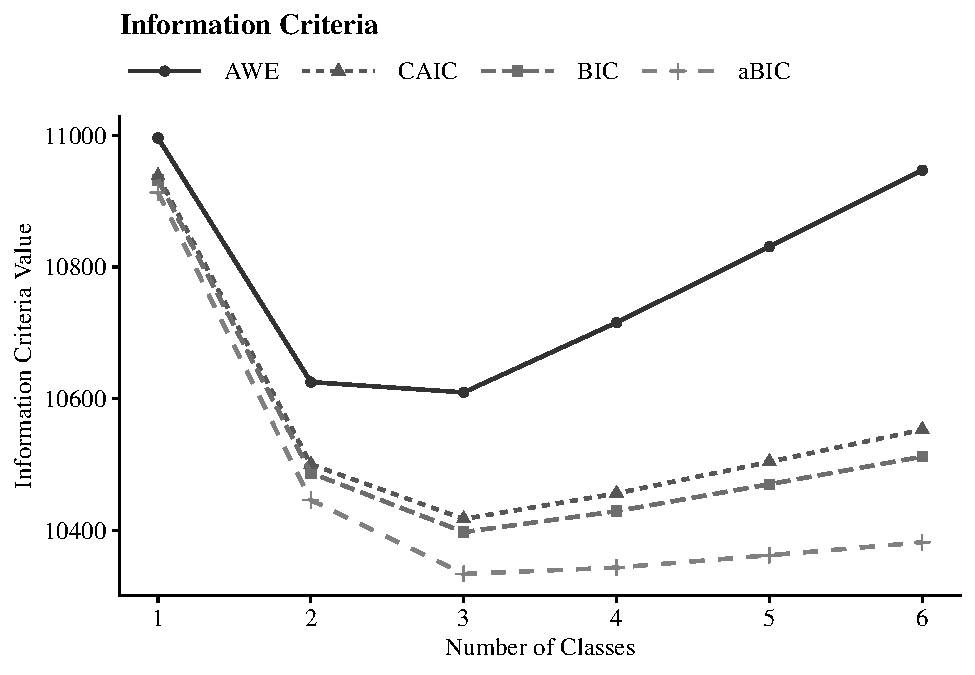
\includegraphics{03-enumeration_files/figure-latex/unnamed-chunk-11-1.pdf}

\begin{center}\rule{0.5\linewidth}{0.5pt}\end{center}

Save figure

\begin{Shaded}
\begin{Highlighting}[]
\FunctionTok{ggsave}\NormalTok{(}\FunctionTok{here}\NormalTok{(}\StringTok{"figures"}\NormalTok{, }\StringTok{"info\_criteria.png"}\NormalTok{), }\AttributeTok{dpi=}\DecValTok{300}\NormalTok{, }\AttributeTok{height=}\DecValTok{5}\NormalTok{, }\AttributeTok{width=}\DecValTok{7}\NormalTok{, }\AttributeTok{units=}\StringTok{"in"}\NormalTok{)}
\end{Highlighting}
\end{Shaded}

\begin{center}\rule{0.5\linewidth}{0.5pt}\end{center}

\section{Compare Class Solutions}\label{compare-class-solutions}

Compare probability plots for \(K = 1:6\) class solutions

\begin{Shaded}
\begin{Highlighting}[]
\NormalTok{model\_results }\OtherTok{\textless{}{-}} \FunctionTok{data.frame}\NormalTok{()}

\ControlFlowTok{for}\NormalTok{ (i }\ControlFlowTok{in} \DecValTok{1}\SpecialCharTok{:}\FunctionTok{length}\NormalTok{(output\_bully)) \{}
  
\NormalTok{  temp }\OtherTok{\textless{}{-}}\NormalTok{ output\_bully[[i]]}\SpecialCharTok{$}\NormalTok{parameters}\SpecialCharTok{$}\NormalTok{probability.scale }\SpecialCharTok{\%\textgreater{}\%}                                       
    \FunctionTok{mutate}\NormalTok{(}\AttributeTok{model =} \FunctionTok{paste}\NormalTok{(i,}\StringTok{"{-}Class Model"}\NormalTok{))                                                  }
  
\NormalTok{  model\_results }\OtherTok{\textless{}{-}} \FunctionTok{rbind}\NormalTok{(model\_results, temp)}
\NormalTok{\}}

\FunctionTok{rm}\NormalTok{(temp)}

\NormalTok{compare\_plot }\OtherTok{\textless{}{-}}
\NormalTok{  model\_results }\SpecialCharTok{\%\textgreater{}\%}
  \FunctionTok{filter}\NormalTok{(category }\SpecialCharTok{==} \DecValTok{2}\NormalTok{) }\SpecialCharTok{\%\textgreater{}\%}
\NormalTok{  dplyr}\SpecialCharTok{::}\FunctionTok{select}\NormalTok{(est, model, LatentClass, param) }\SpecialCharTok{\%\textgreater{}\%}
  \FunctionTok{mutate}\NormalTok{(}\AttributeTok{param =} \FunctionTok{as.factor}\NormalTok{(}\FunctionTok{str\_to\_lower}\NormalTok{(param))) }

\NormalTok{compare\_plot}\SpecialCharTok{$}\NormalTok{param }\OtherTok{\textless{}{-}} \FunctionTok{fct\_inorder}\NormalTok{(compare\_plot}\SpecialCharTok{$}\NormalTok{param)}

\FunctionTok{ggplot}\NormalTok{(}
\NormalTok{  compare\_plot,}
  \FunctionTok{aes}\NormalTok{(}
    \AttributeTok{x =}\NormalTok{ param,}
    \AttributeTok{y =}\NormalTok{ est,}
    \AttributeTok{color =}\NormalTok{ LatentClass,}
    \AttributeTok{shape =}\NormalTok{ LatentClass,}
    \AttributeTok{group =}\NormalTok{ LatentClass,}
    \AttributeTok{lty =}\NormalTok{ LatentClass}
\NormalTok{  )}
\NormalTok{) }\SpecialCharTok{+}
  \FunctionTok{geom\_point}\NormalTok{() }\SpecialCharTok{+} 
  \FunctionTok{geom\_line}\NormalTok{() }\SpecialCharTok{+}
  \FunctionTok{scale\_colour\_viridis\_d}\NormalTok{() }\SpecialCharTok{+}
  \FunctionTok{facet\_wrap}\NormalTok{( }\SpecialCharTok{\textasciitilde{}}\NormalTok{ model, }\AttributeTok{ncol =} \DecValTok{2}\NormalTok{) }\SpecialCharTok{+}
  \FunctionTok{labs}\NormalTok{(}\AttributeTok{title =} \StringTok{"Bullying Items"}\NormalTok{,}
       \AttributeTok{x =} \StringTok{" "}\NormalTok{, }\AttributeTok{y =} \StringTok{"Probability"}\NormalTok{) }\SpecialCharTok{+}
  \FunctionTok{theme\_minimal}\NormalTok{() }\SpecialCharTok{+}
  \FunctionTok{theme}\NormalTok{(}\AttributeTok{panel.grid.major.y =} \FunctionTok{element\_blank}\NormalTok{(),}
                          \AttributeTok{axis.text.x =} \FunctionTok{element\_text}\NormalTok{(}\AttributeTok{angle =} \SpecialCharTok{{-}}\DecValTok{45}\NormalTok{, }\AttributeTok{hjust =} \SpecialCharTok{{-}}\NormalTok{.}\DecValTok{1}\NormalTok{))                            }
\end{Highlighting}
\end{Shaded}

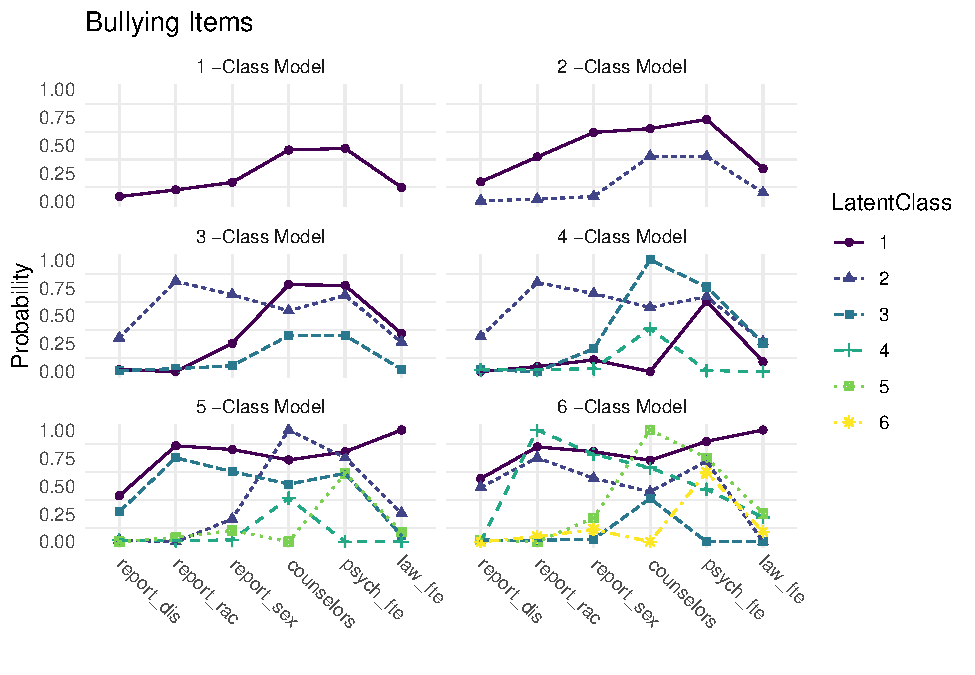
\includegraphics{03-enumeration_files/figure-latex/unnamed-chunk-13-1.pdf}

\begin{center}\rule{0.5\linewidth}{0.5pt}\end{center}

Save figure:

\begin{Shaded}
\begin{Highlighting}[]
\FunctionTok{ggsave}\NormalTok{(}\FunctionTok{here}\NormalTok{(}\StringTok{"figures"}\NormalTok{, }\StringTok{"compare\_kclass\_plot.png"}\NormalTok{), }\AttributeTok{dpi=}\DecValTok{300}\NormalTok{, }\AttributeTok{height=}\DecValTok{5}\NormalTok{, }\AttributeTok{width=}\DecValTok{7}\NormalTok{, }\AttributeTok{units=}\StringTok{"in"}\NormalTok{)}
\end{Highlighting}
\end{Shaded}

\begin{center}\rule{0.5\linewidth}{0.5pt}\end{center}

\section{3-Class Probability Plot}\label{class-probability-plot}

Use the \texttt{plot\_lca} function provided in the folder to plot the item probability plot. This function requires one argument:
- \texttt{model\_name}: The name of the Mplus \texttt{readModels} object (e.g., \texttt{output\_bully\$c3\_bully.out})

\begin{Shaded}
\begin{Highlighting}[]
\FunctionTok{source}\NormalTok{(}\StringTok{"plot\_lca.txt"}\NormalTok{)}

\FunctionTok{plot\_lca}\NormalTok{(}\AttributeTok{model\_name =}\NormalTok{ output\_bully}\SpecialCharTok{$}\NormalTok{c3\_bully.out)}
\end{Highlighting}
\end{Shaded}

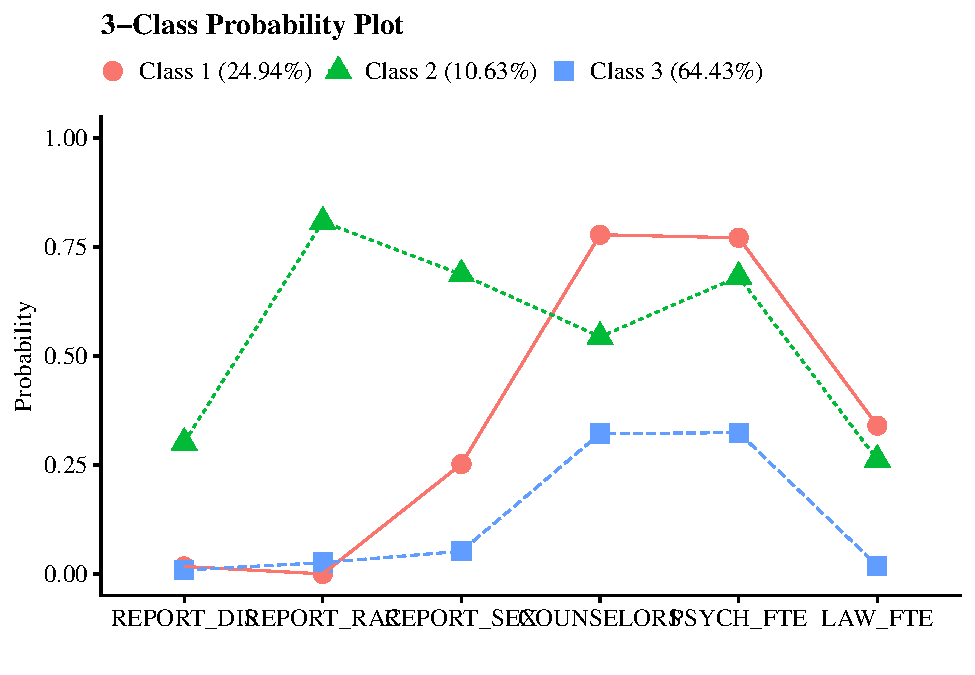
\includegraphics{03-enumeration_files/figure-latex/unnamed-chunk-15-1.pdf}

\begin{center}\rule{0.5\linewidth}{0.5pt}\end{center}

Save figure:

\begin{Shaded}
\begin{Highlighting}[]
\FunctionTok{ggsave}\NormalTok{(}\FunctionTok{here}\NormalTok{(}\StringTok{"figures"}\NormalTok{, }\StringTok{"C3\_bully\_LCA\_Plot.png"}\NormalTok{), }\AttributeTok{dpi=}\StringTok{"retina"}\NormalTok{, }\AttributeTok{height=}\DecValTok{5}\NormalTok{, }\AttributeTok{width=}\DecValTok{7}\NormalTok{, }\AttributeTok{units=}\StringTok{"in"}\NormalTok{)}
\end{Highlighting}
\end{Shaded}

\begin{center}\rule{0.5\linewidth}{0.5pt}\end{center}

\section{Observed Response Patterns}\label{observed-response-patterns}

Save response frequencies for the 3-class model from the previous lab with \texttt{response\ is\ \_\_\_\_\_.dat} under \texttt{SAVEDATA.}

\begin{Shaded}
\begin{Highlighting}[]

\NormalTok{patterns  }\OtherTok{\textless{}{-}} \FunctionTok{mplusObject}\NormalTok{(}
  
  \AttributeTok{TITLE =} \StringTok{"C3 LCA {-} Save response patterns"}\NormalTok{, }
  
  \AttributeTok{VARIABLE =} 
  \StringTok{"categorical = report\_dis{-}law\_fte; }
\StringTok{   usevar =  report\_dis{-}law\_fte;}
\StringTok{   classes = c(3);"}\NormalTok{,}
  
  \AttributeTok{ANALYSIS =} 
   \StringTok{"estimator = mlr; }
\StringTok{    type = mixture;}
\StringTok{    starts = 0;}
\StringTok{    processors = 10;}
\StringTok{    optseed = 802779;"}\NormalTok{,}
  
  \AttributeTok{SAVEDATA =} 
   \StringTok{"File=savedata.dat;}
\StringTok{    Save=cprob;}
\StringTok{    }
\StringTok{    ! Code to save response frequency data }
\StringTok{    }
\StringTok{    response is resp\_patterns.dat;"}\NormalTok{,}
  
  \AttributeTok{OUTPUT =} \StringTok{"residual patterns tech11 tech14"}\NormalTok{,}
  
  \AttributeTok{usevariables =} \FunctionTok{colnames}\NormalTok{(df\_bully),}
  \AttributeTok{rdata =}\NormalTok{ df\_bully)}

\NormalTok{patterns\_fit }\OtherTok{\textless{}{-}} \FunctionTok{mplusModeler}\NormalTok{(patterns,}
                \AttributeTok{dataout=}\FunctionTok{here}\NormalTok{(}\StringTok{"mplus"}\NormalTok{, }\StringTok{"bully.dat"}\NormalTok{),}
                \AttributeTok{modelout=}\FunctionTok{here}\NormalTok{(}\StringTok{"mplus"}\NormalTok{, }\StringTok{"patterns.inp"}\NormalTok{) ,}
                \AttributeTok{check=}\ConstantTok{TRUE}\NormalTok{, }\AttributeTok{run =} \ConstantTok{TRUE}\NormalTok{, }\AttributeTok{hashfilename =} \ConstantTok{FALSE}\NormalTok{)}
\end{Highlighting}
\end{Shaded}

\begin{center}\rule{0.5\linewidth}{0.5pt}\end{center}

Read in observed response pattern data and relabel the columns

\begin{Shaded}
\begin{Highlighting}[]
\CommentTok{\# Read in response frequency data that we just created:}
\NormalTok{patterns }\OtherTok{\textless{}{-}} \FunctionTok{read\_table}\NormalTok{(}\FunctionTok{here}\NormalTok{(}\StringTok{"mplus"}\NormalTok{, }\StringTok{"resp\_patterns.dat"}\NormalTok{),}
                        \AttributeTok{col\_names=}\ConstantTok{FALSE}\NormalTok{, }\AttributeTok{na =} \StringTok{"*"}\NormalTok{) }

\CommentTok{\# Extract the column names}
\NormalTok{names }\OtherTok{\textless{}{-}} \FunctionTok{names}\NormalTok{(}\FunctionTok{readModels}\NormalTok{(}\FunctionTok{here}\NormalTok{(}\StringTok{"mplus"}\NormalTok{, }\StringTok{"patterns.out"}\NormalTok{))[[}\StringTok{\textquotesingle{}savedata\textquotesingle{}}\NormalTok{]]) }

\CommentTok{\# Add the names back to the dataset}
\FunctionTok{colnames}\NormalTok{(patterns) }\OtherTok{\textless{}{-}} \FunctionTok{c}\NormalTok{(}\StringTok{"Frequency"}\NormalTok{, names)  }
\end{Highlighting}
\end{Shaded}

Create a table with the top 5 unconditional response pattern, then top of conditional response pattern for each modal class assignment

\begin{Shaded}
\begin{Highlighting}[]
\CommentTok{\# Order responses by highest frequency}
\NormalTok{order\_highest }\OtherTok{\textless{}{-}}\NormalTok{ patterns }\SpecialCharTok{\%\textgreater{}\%} 
  \FunctionTok{arrange}\NormalTok{(}\FunctionTok{desc}\NormalTok{(Frequency)) }

\CommentTok{\# Loop \textasciigrave{}patterns\textasciigrave{} data to list top 5 conditional response patterns for each class}
\NormalTok{loop\_cond  }\OtherTok{\textless{}{-}} \FunctionTok{lapply}\NormalTok{(}\DecValTok{1}\SpecialCharTok{:}\FunctionTok{max}\NormalTok{(patterns}\SpecialCharTok{$}\NormalTok{C), }\ControlFlowTok{function}\NormalTok{(k) \{       }
\NormalTok{order\_cond }\OtherTok{\textless{}{-}}\NormalTok{ patterns }\SpecialCharTok{\%\textgreater{}\%}                    
  \FunctionTok{filter}\NormalTok{(C }\SpecialCharTok{==}\NormalTok{ k) }\SpecialCharTok{\%\textgreater{}\%}                    
  \FunctionTok{arrange}\NormalTok{(}\FunctionTok{desc}\NormalTok{(Frequency)) }\SpecialCharTok{\%\textgreater{}\%}                
  \FunctionTok{head}\NormalTok{(}\DecValTok{5}\NormalTok{)                                     }
\NormalTok{  \})                                          }

\CommentTok{\# Convert loop into data frame}
\NormalTok{table\_data }\OtherTok{\textless{}{-}} \FunctionTok{as.data.frame}\NormalTok{(}\FunctionTok{bind\_rows}\NormalTok{(loop\_cond))}

\CommentTok{\# Combine unconditional and conditional responses patterns}
\NormalTok{response\_patterns }\OtherTok{\textless{}{-}}  \FunctionTok{rbind}\NormalTok{(order\_highest[}\DecValTok{1}\SpecialCharTok{:}\DecValTok{5}\NormalTok{,], table\_data) }
\end{Highlighting}
\end{Shaded}

Finally, use \texttt{\{gt\}} to make a nicely formatted table

\begin{Shaded}
\begin{Highlighting}[]
\NormalTok{resp\_table }\OtherTok{\textless{}{-}}\NormalTok{ response\_patterns }\SpecialCharTok{\%\textgreater{}\%} 
  \FunctionTok{gt}\NormalTok{() }\SpecialCharTok{\%\textgreater{}\%}
    \FunctionTok{tab\_header}\NormalTok{(}
    \AttributeTok{title =} \StringTok{"Observed Response Patterns"}\NormalTok{,}
    \AttributeTok{subtitle =} \FunctionTok{html}\NormalTok{(}\StringTok{"Response patterns, estimated frequencies, estimated posterior class probabilities and modal assignments"}\NormalTok{)) }\SpecialCharTok{\%\textgreater{}\%} 
    \FunctionTok{tab\_source\_note}\NormalTok{(}
    \AttributeTok{source\_note =} \FunctionTok{md}\NormalTok{(}\StringTok{"Data Source: **Civil Rights Data Collection (CRDC)**"}\NormalTok{)) }\SpecialCharTok{\%\textgreater{}\%}
    \FunctionTok{cols\_label}\NormalTok{(}
      \AttributeTok{Frequency =} \FunctionTok{html}\NormalTok{(}\StringTok{"\textless{}i\textgreater{}f\textless{}/i\textgreater{}\textless{}sub\textgreater{}r\textless{}/sub\textgreater{}"}\NormalTok{),}
    \AttributeTok{REPORT\_D =} \StringTok{"Harrassment: Disability"}\NormalTok{,}
    \AttributeTok{REPORT\_R =} \StringTok{"Harrassment: Race"}\NormalTok{,}
    \AttributeTok{REPORT\_S =} \StringTok{"Harrassment: Sex"}\NormalTok{,}
    \AttributeTok{COUNSELO =} \StringTok{"Staff: Counselor"}\NormalTok{,}
    \AttributeTok{PSYCH\_FT =} \StringTok{"Staff: Psychologist"}\NormalTok{,}
    \AttributeTok{LAW\_FTE =} \StringTok{"Staff: Law Enforcement"}\NormalTok{,}
    \AttributeTok{CPROB1 =} \FunctionTok{html}\NormalTok{(}\StringTok{"P\textless{}sub\textgreater{}\textless{}i\textgreater{}k\textless{}/i\textgreater{}\textless{}/sub\textgreater{}=1"}\NormalTok{),}
    \AttributeTok{CPROB2 =} \FunctionTok{html}\NormalTok{(}\StringTok{"P\textless{}sub\textgreater{}\textless{}i\textgreater{}k\textless{}/i\textgreater{}\textless{}/sub\textgreater{}=2"}\NormalTok{),}
    \AttributeTok{CPROB3 =} \FunctionTok{html}\NormalTok{(}\StringTok{"P\textless{}sub\textgreater{}\textless{}i\textgreater{}k\textless{}/i\textgreater{}\textless{}/sub\textgreater{}=3"}\NormalTok{),}
    \AttributeTok{C =} \FunctionTok{md}\NormalTok{(}\StringTok{"*k*"}\NormalTok{)) }\SpecialCharTok{\%\textgreater{}\%} 
  \FunctionTok{tab\_row\_group}\NormalTok{(}
    \AttributeTok{label =} \StringTok{"Unconditional response patterns"}\NormalTok{,}
    \AttributeTok{rows =} \DecValTok{1}\SpecialCharTok{:}\DecValTok{5}\NormalTok{) }\SpecialCharTok{\%\textgreater{}\%}
  \FunctionTok{tab\_row\_group}\NormalTok{(}
    \AttributeTok{label =} \FunctionTok{md}\NormalTok{(}\StringTok{"*k* = 1 Conditional response patterns"}\NormalTok{),}
    \AttributeTok{rows =} \DecValTok{6}\SpecialCharTok{:}\DecValTok{10}\NormalTok{) }\SpecialCharTok{\%\textgreater{}\%} \CommentTok{\#EDIT THESE VALUES BASED ON THE LAST COLUMN}
  \FunctionTok{tab\_row\_group}\NormalTok{(}
    \AttributeTok{label =} \FunctionTok{md}\NormalTok{(}\StringTok{"*k* = 2 Conditional response patterns"}\NormalTok{),}
    \AttributeTok{rows =} \DecValTok{11}\SpecialCharTok{:}\DecValTok{15}\NormalTok{)  }\SpecialCharTok{\%\textgreater{}\%} \CommentTok{\#EDIT THESE VALUES BASED ON THE LAST COLUMN}
  \FunctionTok{tab\_row\_group}\NormalTok{(}
    \AttributeTok{label =} \FunctionTok{md}\NormalTok{(}\StringTok{"*k* = 3 Conditional response patterns"}\NormalTok{),}
    \AttributeTok{rows =} \DecValTok{16}\SpecialCharTok{:}\DecValTok{20}\NormalTok{)  }\SpecialCharTok{\%\textgreater{}\%} \CommentTok{\#EDIT THESE VALUES BASED ON THE LAST COLUMN  }
    \FunctionTok{row\_group\_order}\NormalTok{(}
      \AttributeTok{groups =} \FunctionTok{c}\NormalTok{(}\StringTok{"Unconditional response patterns"}\NormalTok{,}
                 \FunctionTok{md}\NormalTok{(}\StringTok{"*k* = 1 Conditional response patterns"}\NormalTok{),}
                 \FunctionTok{md}\NormalTok{(}\StringTok{"*k* = 2 Conditional response patterns"}\NormalTok{),}
                 \FunctionTok{md}\NormalTok{(}\StringTok{"*k* = 3 Conditional response patterns"}\NormalTok{))) }\SpecialCharTok{\%\textgreater{}\%} 
    \FunctionTok{tab\_footnote}\NormalTok{(}
    \AttributeTok{footnote =} \FunctionTok{html}\NormalTok{(}
      \StringTok{"\textless{}i\textgreater{}Note.\textless{}/i\textgreater{} \textless{}i\textgreater{}f\textless{}/i\textgreater{}\textless{}sub\textgreater{}r\textless{}/sub\textgreater{} = response pattern frequency; P\textless{}sub\textgreater{}\textless{}i\textgreater{}k\textless{}/i\textgreater{}\textless{}/sub\textgreater{} = posterior class probabilities"}
\NormalTok{    )}
\NormalTok{  ) }\SpecialCharTok{\%\textgreater{}\%} 
  \FunctionTok{cols\_align}\NormalTok{(}\AttributeTok{align =} \StringTok{"center"}\NormalTok{) }\SpecialCharTok{\%\textgreater{}\%} 
  \FunctionTok{opt\_align\_table\_header}\NormalTok{(}\AttributeTok{align =} \StringTok{"left"}\NormalTok{) }\SpecialCharTok{\%\textgreater{}\%} 
\NormalTok{  gt}\SpecialCharTok{::}\FunctionTok{tab\_options}\NormalTok{(}\AttributeTok{table.font.names =} \StringTok{"Times New Roman"}\NormalTok{)}

\NormalTok{resp\_table}
\end{Highlighting}
\end{Shaded}

\begin{table}[!t]
\caption*{
{\large Observed Response Patterns} \\ 
{\small Response patterns, estimated frequencies, estimated posterior class probabilities and modal assignments}
} 
\fontsize{12.0pt}{14.4pt}\selectfont
\begin{tabular*}{\linewidth}{@{\extracolsep{\fill}}ccccccccccc}
\toprule
<i>f</i><sub>r</sub> & Harrassment: Disability & Harrassment: Race & Harrassment: Sex & Staff: Counselor & Staff: Psychologist & Staff: Law Enforcement & P<sub><i>k</i></sub>=1 & P<sub><i>k</i></sub>=2 & P<sub><i>k</i></sub>=3 & \emph{k} \\ 
\midrule\addlinespace[2.5pt]
\multicolumn{11}{l}{Unconditional response patterns} \\[2.5pt] 
\midrule\addlinespace[2.5pt]
525 & 0 & 0 & 0 & 0 & 0 & 0 & 0.023 & 0.002 & 0.976 & 3 \\ 
299 & 0 & 0 & 0 & 0 & 1 & 0 & 0.139 & 0.007 & 0.854 & 3 \\ 
293 & 0 & 0 & 0 & 1 & 0 & 0 & 0.146 & 0.004 & 0.850 & 3 \\ 
251 & 0 & 0 & 0 & 1 & 1 & 0 & 0.541 & 0.009 & 0.449 & 1 \\ 
75 & 0 & 0 & 0 & 1 & 1 & 1 & 0.959 & 0.011 & 0.030 & 1 \\ 
\midrule\addlinespace[2.5pt]
\multicolumn{11}{l}{\emph{k} = 1 Conditional response patterns} \\[2.5pt] 
\midrule\addlinespace[2.5pt]
251 & 0 & 0 & 0 & 1 & 1 & 0 & 0.541 & 0.009 & 0.449 & 1 \\ 
75 & 0 & 0 & 0 & 1 & 1 & 1 & 0.959 & 0.011 & 0.030 & 1 \\ 
72 & 0 & 0 & 1 & 1 & 1 & 0 & 0.803 & 0.088 & 0.108 & 1 \\ 
38 & 0 & 0 & 1 & 0 & 1 & 0 & 0.431 & 0.139 & 0.430 & 1 \\ 
34 & 0 & 0 & 0 & 0 & 1 & 1 & 0.789 & 0.027 & 0.184 & 1 \\ 
\midrule\addlinespace[2.5pt]
\multicolumn{11}{l}{\emph{k} = 2 Conditional response patterns} \\[2.5pt] 
\midrule\addlinespace[2.5pt]
24 & 0 & 1 & 0 & 0 & 1 & 0 & 0.000 & 0.561 & 0.439 & 2 \\ 
20 & 0 & 1 & 1 & 0 & 1 & 0 & 0.000 & 0.981 & 0.019 & 2 \\ 
19 & 0 & 1 & 1 & 1 & 1 & 0 & 0.000 & 0.992 & 0.008 & 2 \\ 
18 & 0 & 1 & 1 & 1 & 0 & 0 & 0.000 & 0.967 & 0.033 & 2 \\ 
12 & 0 & 1 & 1 & 1 & 1 & 1 & 0.000 & 1.000 & 0.000 & 2 \\ 
\midrule\addlinespace[2.5pt]
\multicolumn{11}{l}{\emph{k} = 3 Conditional response patterns} \\[2.5pt] 
\midrule\addlinespace[2.5pt]
525 & 0 & 0 & 0 & 0 & 0 & 0 & 0.023 & 0.002 & 0.976 & 3 \\ 
299 & 0 & 0 & 0 & 0 & 1 & 0 & 0.139 & 0.007 & 0.854 & 3 \\ 
293 & 0 & 0 & 0 & 1 & 0 & 0 & 0.146 & 0.004 & 0.850 & 3 \\ 
36 & 0 & 0 & 1 & 0 & 0 & 0 & 0.117 & 0.060 & 0.823 & 3 \\ 
27 & 0 & 0 & 0 & NA & NA & NA & 0.236 & 0.006 & 0.758 & 3 \\ 
\bottomrule
\end{tabular*}
\begin{minipage}{\linewidth}
<i>Note.</i> <i>f</i><sub>r</sub> = response pattern frequency; P<sub><i>k</i></sub> = posterior class probabilities\\
Data Source: \textbf{Civil Rights Data Collection (CRDC)}\\
\end{minipage}
\end{table}

\begin{center}\rule{0.5\linewidth}{0.5pt}\end{center}

Save table:

\begin{Shaded}
\begin{Highlighting}[]
\FunctionTok{gtsave}\NormalTok{(resp\_table, }\FunctionTok{here}\NormalTok{(}\StringTok{"figures"}\NormalTok{,}\StringTok{"resp\_table.png"}\NormalTok{))}
\end{Highlighting}
\end{Shaded}

\begin{center}\rule{0.5\linewidth}{0.5pt}\end{center}

\section{Classification Diagnostics}\label{classification-diagnostics}

Use Mplus to calculate k-class confidence intervals (Note: Change the synax to make your chosen \emph{k}-class model):

\begin{Shaded}
\begin{Highlighting}[]
\NormalTok{classification  }\OtherTok{\textless{}{-}} \FunctionTok{mplusObject}\NormalTok{(}
  
  \AttributeTok{TITLE =} \StringTok{"C3 LCA {-} Calculated k{-}Class 95\% CI"}\NormalTok{,}
  
  \AttributeTok{VARIABLE =}
    \StringTok{"categorical = report\_dis{-}law\_fte;}
\StringTok{   usevar =  report\_dis{-}law\_fte;}
\StringTok{   classes = c(3);"}\NormalTok{, }
  
  \AttributeTok{ANALYSIS =}
    \StringTok{"estimator = ml;}
\StringTok{    type = mixture;}
\StringTok{    starts = 0; }
\StringTok{    processors = 10;}
\StringTok{    optseed = 802779;}
\StringTok{    bootstrap = 1000;"}\NormalTok{,}
  
  \AttributeTok{MODEL =}
    \StringTok{"}
\StringTok{  !CHANGE THIS SECTION TO YOUR CHOSEN k{-}CLASS MODEL}
\StringTok{    }
\StringTok{  \%OVERALL\%}
\StringTok{  [C\#1](c1);}
\StringTok{  }
\StringTok{  [C\#2](C2);}

\StringTok{  Model Constraint:}
\StringTok{  New(p1 p2 p3);}
\StringTok{  }
\StringTok{  p1 = exp(c1)/(1+exp(c1)+exp(c2));}
\StringTok{  p2 = exp(c2)/(1+exp(c1)+exp(c2));}
\StringTok{  p3 = 1/(1+exp(c1)+exp(c2));"}\NormalTok{,}

  
  \AttributeTok{OUTPUT =} \StringTok{"cinterval(bcbootstrap)"}\NormalTok{,}
  
  \AttributeTok{usevariables =} \FunctionTok{colnames}\NormalTok{(df\_bully),}
  \AttributeTok{rdata =}\NormalTok{ df\_bully)}

\NormalTok{classification\_fit }\OtherTok{\textless{}{-}} \FunctionTok{mplusModeler}\NormalTok{(classification,}
                \AttributeTok{dataout=}\FunctionTok{here}\NormalTok{(}\StringTok{"mplus"}\NormalTok{, }\StringTok{"bully.dat"}\NormalTok{),}
                \AttributeTok{modelout=}\FunctionTok{here}\NormalTok{(}\StringTok{"mplus"}\NormalTok{, }\StringTok{"class.inp"}\NormalTok{) ,}
                \AttributeTok{check=}\ConstantTok{TRUE}\NormalTok{, }\AttributeTok{run =} \ConstantTok{TRUE}\NormalTok{, }\AttributeTok{hashfilename =} \ConstantTok{FALSE}\NormalTok{)}
\end{Highlighting}
\end{Shaded}

\emph{Note}: Ensure that the classes did not shift during this step (i.g., Class 1 in the enumeration run is now Class 4). Evaluate output and compare the class counts and proportions for the latent classes. Using the OPTSEED function ensures replication of the best loglikelihood value run.

\begin{center}\rule{0.5\linewidth}{0.5pt}\end{center}

Read in the 3-class model:

\begin{Shaded}
\begin{Highlighting}[]
\CommentTok{\# Read in the 3{-}class model and extract information needed}
\NormalTok{output\_bully }\OtherTok{\textless{}{-}} \FunctionTok{readModels}\NormalTok{(}\FunctionTok{here}\NormalTok{(}\StringTok{"mplus"}\NormalTok{, }\StringTok{"class.out"}\NormalTok{))}

\CommentTok{\# Entropy}
\NormalTok{entropy }\OtherTok{\textless{}{-}} \FunctionTok{c}\NormalTok{(output\_bully}\SpecialCharTok{$}\NormalTok{summaries}\SpecialCharTok{$}\NormalTok{Entropy, }\FunctionTok{rep}\NormalTok{(}\ConstantTok{NA}\NormalTok{, output\_bully}\SpecialCharTok{$}\NormalTok{summaries}\SpecialCharTok{$}\NormalTok{NLatentClasses}\DecValTok{{-}1}\NormalTok{))}

\CommentTok{\# 95\% k{-}Class and k{-}class 95\% Confidence Intervals}
\NormalTok{k\_ci }\OtherTok{\textless{}{-}}\NormalTok{ output\_bully}\SpecialCharTok{$}\NormalTok{parameters}\SpecialCharTok{$}\NormalTok{ci.unstandardized }\SpecialCharTok{\%\textgreater{}\%} 
  \FunctionTok{filter}\NormalTok{(paramHeader }\SpecialCharTok{==} \StringTok{"New.Additional.Parameters"}\NormalTok{) }\SpecialCharTok{\%\textgreater{}\%} 
  \FunctionTok{unite}\NormalTok{(CI, }\FunctionTok{c}\NormalTok{(low2}\FloatTok{.5}\NormalTok{,up2}\FloatTok{.5}\NormalTok{), }\AttributeTok{sep=}\StringTok{", "}\NormalTok{, }\AttributeTok{remove =} \ConstantTok{TRUE}\NormalTok{) }\SpecialCharTok{\%\textgreater{}\%} 
  \FunctionTok{mutate}\NormalTok{(}\AttributeTok{CI =} \FunctionTok{paste0}\NormalTok{(}\StringTok{"["}\NormalTok{, CI, }\StringTok{"]"}\NormalTok{)) }\SpecialCharTok{\%\textgreater{}\%} 
  \FunctionTok{rename}\NormalTok{(}\AttributeTok{kclass=}\NormalTok{est) }\SpecialCharTok{\%\textgreater{}\%} 
\NormalTok{  dplyr}\SpecialCharTok{::}\FunctionTok{select}\NormalTok{(kclass, CI)}

\CommentTok{\# AvePPk = Average Latent Class Probabilities for Most Likely Latent Class Membership (Row) by Latent Class (Column)}
\NormalTok{avePPk }\OtherTok{\textless{}{-}} \FunctionTok{tibble}\NormalTok{(}\AttributeTok{avePPk =} \FunctionTok{diag}\NormalTok{(output\_bully}\SpecialCharTok{$}\NormalTok{class\_counts}\SpecialCharTok{$}\NormalTok{avgProbs.mostLikely))}

\CommentTok{\# mcaPk = modal class assignment proportion }
\NormalTok{mcaPk }\OtherTok{\textless{}{-}} \FunctionTok{round}\NormalTok{(output\_bully}\SpecialCharTok{$}\NormalTok{class\_counts}\SpecialCharTok{$}\NormalTok{mostLikely,}\DecValTok{3}\NormalTok{) }\SpecialCharTok{\%\textgreater{}\%} 
  \FunctionTok{mutate}\NormalTok{(}\AttributeTok{model =} \FunctionTok{paste0}\NormalTok{(}\StringTok{"Class "}\NormalTok{, class)) }\SpecialCharTok{\%\textgreater{}\%} 
  \FunctionTok{add\_column}\NormalTok{(avePPk, k\_ci) }\SpecialCharTok{\%\textgreater{}\%} 
  \FunctionTok{rename}\NormalTok{(}\AttributeTok{mcaPk =}\NormalTok{ proportion) }\SpecialCharTok{\%\textgreater{}\%} 
\NormalTok{  dplyr}\SpecialCharTok{::}\FunctionTok{select}\NormalTok{(model, kclass, CI, mcaPk, avePPk)}

\CommentTok{\# OCCk = odds of correct classification}
\NormalTok{OCCk }\OtherTok{\textless{}{-}}\NormalTok{ mcaPk }\SpecialCharTok{\%\textgreater{}\%} 
  \FunctionTok{mutate}\NormalTok{(}\AttributeTok{OCCk =} \FunctionTok{round}\NormalTok{((avePPk}\SpecialCharTok{/}\NormalTok{(}\DecValTok{1}\SpecialCharTok{{-}}\NormalTok{avePPk))}\SpecialCharTok{/}\NormalTok{(kclass}\SpecialCharTok{/}\NormalTok{(}\DecValTok{1}\SpecialCharTok{{-}}\NormalTok{kclass)),}\DecValTok{3}\NormalTok{))}

\CommentTok{\# Put everything together}
\NormalTok{class\_table }\OtherTok{\textless{}{-}} \FunctionTok{data.frame}\NormalTok{(OCCk, entropy)}
\end{Highlighting}
\end{Shaded}

Now, use \texttt{\{gt\}} to make a nicely formatted table

\begin{Shaded}
\begin{Highlighting}[]
\NormalTok{class\_table }\OtherTok{\textless{}{-}}\NormalTok{ class\_table }\SpecialCharTok{\%\textgreater{}\%} 
  \FunctionTok{gt}\NormalTok{() }\SpecialCharTok{\%\textgreater{}\%}
    \FunctionTok{tab\_header}\NormalTok{(}
    \AttributeTok{title =} \StringTok{"Model Classification Diagnostics for the 3{-}Class Solution"}\NormalTok{) }\SpecialCharTok{\%\textgreater{}\%}
    \FunctionTok{cols\_label}\NormalTok{(}
      \AttributeTok{model =} \FunctionTok{md}\NormalTok{(}\StringTok{"*k*{-}Class"}\NormalTok{),}
      \AttributeTok{kclass =} \FunctionTok{md}\NormalTok{(}\StringTok{"*k*{-}Class Proportions"}\NormalTok{),}
      \AttributeTok{CI =} \StringTok{"95\% CI"}\NormalTok{,}
      \AttributeTok{mcaPk =} \FunctionTok{html}\NormalTok{(}\StringTok{"McaP\textless{}sub\textgreater{}k\textless{}/sub\textgreater{}"}\NormalTok{),}
      \AttributeTok{avePPk =} \FunctionTok{md}\NormalTok{(}\StringTok{"AvePP\textless{}sub\textgreater{}k\textless{}/sub\textgreater{}"}\NormalTok{),}
      \AttributeTok{OCCk =} \FunctionTok{md}\NormalTok{(}\StringTok{"OCC\textless{}sub\textgreater{}k\textless{}/sub\textgreater{}"}\NormalTok{),}
      \AttributeTok{entropy =} \StringTok{"Entropy"}\NormalTok{) }\SpecialCharTok{\%\textgreater{}\%} 
    \FunctionTok{sub\_missing}\NormalTok{(}\DecValTok{7}\NormalTok{,}
              \AttributeTok{missing\_text =} \StringTok{""}\NormalTok{) }\SpecialCharTok{\%\textgreater{}\%}
    \FunctionTok{tab\_footnote}\NormalTok{(}
    \AttributeTok{footnote =} \FunctionTok{html}\NormalTok{(}
      \StringTok{"\textless{}i\textgreater{}Note.\textless{}/i\textgreater{} McaP\textless{}sub\textgreater{}k\textless{}/sub\textgreater{} = Modal class assignment proportion; AvePP\textless{}sub\textgreater{}k\textless{}/sub\textgreater{} = Average posterior class probabilities; OCC\textless{}sub\textgreater{}k\textless{}/sub\textgreater{} = Odds of correct classification; "}
\NormalTok{    )}
\NormalTok{  ) }\SpecialCharTok{\%\textgreater{}\%} 
  \FunctionTok{cols\_align}\NormalTok{(}\AttributeTok{align =} \StringTok{"center"}\NormalTok{) }\SpecialCharTok{\%\textgreater{}\%} 
  \FunctionTok{opt\_align\_table\_header}\NormalTok{(}\AttributeTok{align =} \StringTok{"left"}\NormalTok{) }\SpecialCharTok{\%\textgreater{}\%} 
\NormalTok{  gt}\SpecialCharTok{::}\FunctionTok{tab\_options}\NormalTok{(}\AttributeTok{table.font.names =} \StringTok{"Times New Roman"}\NormalTok{)}

\NormalTok{class\_table}
\end{Highlighting}
\end{Shaded}

\begin{table}[!t]
\caption*{
{\large Model Classification Diagnostics for the 3-Class Solution}
} 
\fontsize{12.0pt}{14.4pt}\selectfont
\begin{tabular*}{\linewidth}{@{\extracolsep{\fill}}ccccccc}
\toprule
\emph{k}-Class & \emph{k}-Class Proportions & 95\% CI & McaP<sub>k</sub> & AvePPk & OCCk & Entropy \\ 
\midrule\addlinespace[2.5pt]
Class 1 & 0.249 & [0.166, 0.329] & 0.282 & 0.675 & 6.264 & 0.635 \\ 
Class 2 & 0.106 & [0.083, 0.136] & 0.095 & 0.904 & 79.420 &  \\ 
Class 3 & 0.644 & [0.561, 0.731] & 0.623 & 0.893 & 4.614 &  \\ 
\bottomrule
\end{tabular*}
\begin{minipage}{\linewidth}
<i>Note.</i> McaP<sub>k</sub> = Modal class assignment proportion; AvePP<sub>k</sub> = Average posterior class probabilities; OCC<sub>k</sub> = Odds of correct classification; \\
\end{minipage}
\end{table}

  \bibliography{book.bib,packages.bib}

\end{document}
